%% Time-stamp: <2019-03-01 13:49:57 (marc)>
\documentclass[xcolor=x11names,compress, mathserif,xcolor=table]{beamer}
\newcommand\hmmax{0}
\newcommand\bmmax{0}

\newcommand{\hackspace}{\hspace{4.2mm}}
\newcommand{\showstudent}[1]{}





% talk/author information
\newcommand{\authorname}{Mark van der Wilk}
\newcommand{\authoremail}{m.vdwilk@imperial.ac.uk}
\newcommand{\authoraffiliation}{
 Department of Computing\\Imperial
  College London}
\newcommand{\authortwitter}{markvanderwilk}
\newcommand{\slidesettitle}{\imperialBlue{Variational Inference}}
\newcommand{\footertitle}{Variational Inference}
\newcommand{\location}{Imperial College}
\newcommand{\talkDate}{February 27, 2023}

\newcommand{\lb}{\mathcal{L}}



\date{\imperialGray{\talkDate}}

\usepackage{../includes/MarkMathCmds}



% load defaults
\selectcolormodel{rgb}
\usepackage{ifxetex,ifluatex}
\newif\ifxetexorluatex
\ifxetex
  \xetexorluatextrue
\else
  \ifluatex
    \xetexorluatextrue
  \else
    \xetexorluatexfalse
  \fi
\fi

\usepackage{textpos}
%\usepackage{arabtex}
\usepackage{tikz}
\usetikzlibrary{decorations.markings}
\usetikzlibrary{arrows}
\usetikzlibrary{shapes}
\usetikzlibrary{plotmarks}
\usetikzlibrary{mindmap,trees,backgrounds}

\tikzstyle{every picture}+=[remember picture]

%\usepackage{movie15}
% \usepackage{pdfpages}
%\usepackage{xmpmulti}

\usepackage{anyfontsize}
\usepackage{wrapfig}
\usepackage{animate}
\usepackage{multirow}
\usepackage{multimedia}
\usepackage{xmpmulti}
%\usepackage[latin9]{inputenc}
\usepackage[english]{babel}
\usepackage{scalefnt}
\usepackage{verbatim}
\usepackage{url}
% \usepackage{pgf,pgfarrows,pgfnodes}
\usepackage{textpos}
\usepackage[tight,ugly]{units}
\usepackage{url}
\usepackage{bbm}
\usepackage[english]{babel}
\usepackage{fancyhdr}
\usepackage{bm} % correct bold symbols, like \bm
\usepackage{amsmath}
\usepackage{amsfonts}
\usepackage{amssymb}
\usepackage{mathrsfs}
\usepackage{mathtools}
\usepackage{color}
\usepackage{cancel}
\usepackage{algorithm}
\usepackage{algpseudocode}
\usepackage{mathrsfs}
\usepackage{listings}
\usepackage{graphicx} % for pdf, bitmapped graphics files
\usepackage{mathtools}
\usepackage{units}
\usepackage{subfig}
\usepackage{enumerate}
\usepackage{natbib}
\usepackage{dsfont}


\ifxetexorluatex
\usepackage{fontspec}
\setmainfont[Scale=0.8]{OpenDyslexic-Regular}
\else
\usefonttheme{professionalfonts}
\fi

\renewcommand{\vec}[1]{{\boldsymbol{{#1}}}} % vector
\newcommand{\mat}[1]{{\boldsymbol{{#1}}}} % matrix
% \newcommand{\KL}[2]{\mathrm{KL}(#1\|#2)} % KL divergence
\newcommand{\R}[0]{\mathds{R}} % real numbers
\newcommand{\Z}[0]{\mathds{Z}} % integers
\newcommand{\tr}[0]{\text{tr}} % trace
% \newcommand{\inv}{^{-1}}
% \DeclareMathOperator*{\diag}{diag}
\newcommand{\E}{\mathds{E}} % expectation
\newcommand{\var}{\mathds{V}}
\newcommand{\gauss}[2]{\mathcal{N}\big(#1,\,#2\big)}
\newcommand{\gaussx}[3]{\mathcal{N}\big(#1\,|\,#2,\,#3\big)}
\newcommand{\gaussBig}[2]{\mathcal{N}\left(#1,\,#2\right)}
\newcommand{\gaussxBig}[3]{\mathcal{N}\left(#1\,\left|\,#2,\,#3\right.\right)}
\newcommand{\Ber}[0]{\mathrm{Ber}} % Bernoulli distribution
\DeclareMathOperator{\cov}{Cov}
\ifxetexorluatex
\renewcommand{\T}[0]{^\top}
\renewcommand{\d}[0]{\text{d}} % derivative
\else
\newcommand{\T}[0]{^\top}
\renewcommand{\d}[0]{\text{d}} % derivative
\fi
% calculus
\newcommand{\pdiff}[1]{\frac{\partial}{\partial #1}}
\newcommand{\pdiffF}[2]{\frac{\partial #1}{\partial #2}}
\newcommand{\diffF}[2]{\frac{{\d}#1}{{\d}#2}}
\newcommand{\diffFII}[2]{\frac{{\d}^2 #1}{{\d}#2^2}}
\newcommand{\diff}[1]{\frac{{\d}}{{\d}#1}}
\newcommand{\diffII}[1]{\frac{{\d}^2}{{\d}#1^2}}
\newcommand{\class}[0]{\mathcal{C}}

\newcommand{\idx}[1]{^{(#1)}}
% \newcommand{\norm}[1]{\left\|#1\right\|}
\newcommand{\proj}[1]{\tilde{#1}}
\newcommand{\pcacoord}{z}
\newcommand{\pcacoordnew}{\zeta}
\newcommand{\latent}{z}
% \newcommand{\given}{\,|\,}
\newcommand{\genset}[1]{\mathrm{span}[#1]} % generating set
\newcommand{\set}[1]{\mathcal{#1}} % set
\newcommand{\fixgmfont}[1]{\scalebox{0.8}{#1}}



\usepackage{pifont}% http://ctan.org/pkg/pifont
\newcommand{\cmark}{{\color{green!40!black}\ding{51}}}%
\newcommand{\xmark}{{\color{red}\ding{55}}}%
\newcommand{\green}[1]{{\bf{\textcolor{green}{#1}}}}
\newcommand{\red}[1]{{\bf{\textcolor{red}{#1}}}}

\newcommand<>\red[1]{{\color#2[rgb]{1,0,0}#1}}
\newcommand<>\blue[1]{{\color#2[rgb]{0,0,1}#1}}
\newcommand<>\yellow[1]{{\color#2{camyellow}#1}}
\newcommand<>\green[1]{{\color#2[rgb]{0,0.6,0.0}#1}}
\newcommand<>\violet[1]{{\color#2[rgb]{0.6,0,0.6}#1}}
\newcommand<>\orange[1]{{\color#2[rgb]{1,0.5,0}#1}}
\newcommand<>\black[1]{{\color#2[rgb]{0,0,0}#1}}
\newcommand<>\steel[1]{{\color#2[rgb]{0,0,0.8}#1}}
\newcommand<>\darkblue[1]{{\color#2[rgb]{0,0,0.6}#1}}
\newcommand<>\lightblue[1]{{\color#2[rgb]{0.4,0.4,0.7}#1}}
\newcommand<>\gray[1]{{\color#2[rgb]{0.4,0.4,0.4}#1}}
\newcommand<>\greenish[1]{{\color#2[rgb]{0.45, 0.66, 0.45}#1}}
\newcommand<>\redish[1]{{\color#2[rgb]{0.7843    0.3706    0.3706}#1}}
\definecolor{redishTIKZ}{rgb}{0.7843, 0.3706, 0.3706}
\definecolor{imperialBlue}{rgb}{0.058, 0.219, 0.418}
\definecolor{aimsbrown}{rgb}{0.539, 0.117, 0.015}
% \definecolor{imperialGray}{rgb}{0.414, 0.488, 0.671 }
\definecolor{imperialGray}{RGB}{109,153, 204}
\definecolor{aimslightbrown}{RGB}{138,88,84}
\newcommand<>\imperialBlue[1]{{\color#2[rgb]{0.058, 0.219, 0.418}#1}}
\newcommand<>\aimsbrown[1]{{\color#2[rgb]{0.539, 0.117, 0.015}#1}}
%\newcommand<>\imperialGray[1]{{\color#2[rgb]{0.414, 0.488, 0.671}#1}}
\newcommand<>\imperialGray[1]{{\color#2[RGB]{109,153, 204}#1}}
\newcommand<>\aimslightbrown[1]{{\color#2[RGB]{138,88,84}#1}}
\newcommand<>\lightgray[1]{{\color#2[rgb]{0.8,0.8,0.8}#1}}
%\newcommand<>\highlightcolor[1]{{\color#2[rgb]{0,0,1}#1}}
\newcommand{\highlight}[1]{{\bf\steel{#1}}}
%\newcommand{\newblock}[0]{}

%\newcommand{\arrow}[0]{\includegraphics[height=5pt]{./figures/arrow}\hspace{3pt}}

\renewcommand{\emph}[1]{\textbf{\steel{{#1}}}}

\renewcommand{\alert}[1]{{\bf\red{{#1}}}}

\newcommand{\arrow}{
\begin{tikzpicture}
\draw [black!40!green, fill=black!40!green] (0,-0.12) -- (0,0.12) --
(0.15,0);
\draw [black!40!green, fill=black!40!green] (0.15,-0.12) -- (0.15,0.12) --
(0.3,0); 
\end{tikzpicture}
}

\geometry{left=0.45cm,top=0cm,right=0.45cm}


\newcommand{\logoimagepath}{./figures/imperial}
\newcommand{\highlightcolor}{blue!80!black}
%\newcommand{\headbarcolor}{imperialBlue}
\newcommand{\headbarcolor}{imperialBlue}
\institute{}

\newcommand{\coursetitle}{}

\newcommand{\slidesetsubtitle}{}
\newcommand{\slidesetnumber}{01}
\usefonttheme{professionalfonts}


\usetikzlibrary{decorations.fractals}
% tikzlibrary.code.tex
%
% Copyright 2010-2011 by Laura Dietz
% Copyright 2012 by Jaakko Luttinen
%
% The MIT License
%
% See LICENSE file for more details.

% Load other libraries
\usetikzlibrary{shapes}
\usetikzlibrary{fit}
\usetikzlibrary{chains}
\usetikzlibrary{arrows}

% Latent node
\tikzstyle{latent} = [circle,fill=white,draw=black,inner sep=1pt,
minimum size=20pt, font=\fontsize{10}{10}\selectfont, node distance=1]
% Observed node
\tikzstyle{obs} = [latent,fill=gray!25]
% Constant node
\tikzstyle{const} = [rectangle, inner sep=0pt, node distance=1]
% Factor node
\tikzstyle{factor} = [rectangle, fill=black,minimum size=5pt, inner
sep=0pt, node distance=0.4]
% Deterministic node
\tikzstyle{det} = [latent, diamond]

% Plate node
\tikzstyle{plate} = [draw, rectangle, rounded corners, fit=#1]
% Invisible wrapper node
\tikzstyle{wrap} = [inner sep=0pt, fit=#1]
% Gate
\tikzstyle{gate} = [draw, rectangle, dashed, fit=#1]

% Caption node
\tikzstyle{caption} = [font=\footnotesize, node distance=0] %
\tikzstyle{plate caption} = [caption, node distance=0, inner sep=0pt,
below left=5pt and 0pt of #1.south east] %
\tikzstyle{factor caption} = [caption] %
\tikzstyle{every label} += [caption] %

%\pgfdeclarelayer{b}
%\pgfdeclarelayer{f}
%\pgfsetlayers{b,main,f}

% \factoredge [options] {inputs} {factors} {outputs}
\newcommand{\factoredge}[4][]{ %
  % Connect all nodes #2 to all nodes #4 via all factors #3.
  \foreach \f in {#3} { %
    \foreach \x in {#2} { %
      \path (\x) edge[-,#1] (\f) ; %
      %\draw[-,#1] (\x) edge[-] (\f) ; %
    } ;
    \foreach \y in {#4} { %
      \path (\f) edge[->, >={triangle 45}, #1] (\y) ; %
      %\draw[->,#1] (\f) -- (\y) ; %
    } ;
  } ;
}

% \edge [options] {inputs} {outputs}
\newcommand{\edge}[3][]{ %
  % Connect all nodes #2 to all nodes #3.
  \foreach \x in {#2} { %
    \foreach \y in {#3} { %
      \path (\x) edge [->, >={triangle 45}, #1] (\y) ;%
      %\draw[->,#1] (\x) -- (\y) ;%
    } ;
  } ;
}

% \factor [options] {name} {caption} {inputs} {outputs}
\newcommand{\factor}[5][]{ %
  % Draw the factor node. Use alias to allow empty names.
  \node[factor, label={[name=#2-caption]#3}, name=#2, #1,
  alias=#2-alias] {} ; %
  % Connect all inputs to outputs via this factor
  \factoredge {#4} {#2-alias} {#5} ; %
}

% \plate [options] {name} {fitlist} {caption}
\newcommand{\plate}[4][]{ %
  \node[wrap=#3] (#2-wrap) {}; %
  \node[plate caption=#2-wrap] (#2-caption) {#4}; %
  \node[plate=(#2-wrap)(#2-caption), #1] (#2) {}; %
}

% \gate [options] {name} {fitlist} {inputs}
\newcommand{\gate}[4][]{ %
  \node[gate=#3, name=#2, #1, alias=#2-alias] {}; %
  \foreach \x in {#4} { %
    \draw [-*,thick] (\x) -- (#2-alias); %
  } ;%
}

% \vgate {name} {fitlist-left} {caption-left} {fitlist-right}
% {caption-right} {inputs}
\newcommand{\vgate}[6]{ %
  % Wrap the left and right parts
  \node[wrap=#2] (#1-left) {}; %
  \node[wrap=#4] (#1-right) {}; %
  % Draw the gate
  \node[gate=(#1-left)(#1-right)] (#1) {}; %
  % Add captions
  \node[caption, below left=of #1.north ] (#1-left-caption)
  {#3}; %
  \node[caption, below right=of #1.north ] (#1-right-caption)
  {#5}; %
  % Draw middle separation
  \draw [-, dashed] (#1.north) -- (#1.south); %
  % Draw inputs
  \foreach \x in {#6} { %
    \draw [-*,thick] (\x) -- (#1); %
  } ;%
}

% \hgate {name} {fitlist-top} {caption-top} {fitlist-bottom}
% {caption-bottom} {inputs}
\newcommand{\hgate}[6]{ %
  % Wrap the left and right parts
  \node[wrap=#2] (#1-top) {}; %
  \node[wrap=#4] (#1-bottom) {}; %
  % Draw the gate
  \node[gate=(#1-top)(#1-bottom)] (#1) {}; %
  % Add captions
  \node[caption, above right=of #1.west ] (#1-top-caption)
  {#3}; %
  \node[caption, below right=of #1.west ] (#1-bottom-caption)
  {#5}; %
  % Draw middle separation
  \draw [-, dashed] (#1.west) -- (#1.east); %
  % Draw inputs
  \foreach \x in {#6} { %
    \draw [-*,thick] (\x) -- (#1); %
  } ;%
}


% Copyright (C) 2016  Joseph Rabinoff

% ipe2tikz is free software; you can redistribute it and/or modify it under
% the terms of the GNU General Public License as published by the Free
% Software Foundation; either version 3 of the License, or (at your option)
% any later version.

% ipe2tikz is distributed in the hope that it will be useful, but WITHOUT ANY
% WARRANTY; without even the implied warranty of MERCHANTABILITY or FITNESS
% FOR A PARTICULAR PURPOSE.  See the GNU General Public License for more
% details.

% You should have received a copy of the GNU General Public License along with
% ipe2tikz; if not, you can find it at "http://www.gnu.org/copyleft/gpl.html",
% or write to the Free Software Foundation, Inc., 675 Mass Ave, Cambridge, MA
% 02139, USA.


% ipe compatibility TikZ styles

\usetikzlibrary{arrows.meta}

\makeatletter

% These should behave almost exactly like ipe arrows.  They disable correcting
% for the miter length and line width.  This is important for visual consistency
% with ipe, since ipe arrows get much larger when the line width is increased.
% They also use the line join and cap styles from the main path.  These are very
% simple arrows: there is no harpoon version, and the convex hull computation is
% sloppy.

\pgfdeclarearrow{
  name = ipe _linear,
  defaults = {
    length = +1bp,
    width  = +.666bp,
    line width = +0pt 1,
  },
  setup code = {
    % Control points
    \pgfarrowssetbackend{0pt}
    \pgfarrowssetvisualbackend{
      \pgfarrowlength\advance\pgf@x by-.5\pgfarrowlinewidth}
    \pgfarrowssetlineend{\pgfarrowlength}
    \ifpgfarrowreversed
      \pgfarrowssetlineend{\pgfarrowlength\advance\pgf@x by-.5\pgfarrowlinewidth}
    \fi
    \pgfarrowssettipend{\pgfarrowlength}
    % Convex hull
    \pgfarrowshullpoint{\pgfarrowlength}{0pt}
    \pgfarrowsupperhullpoint{0pt}{.5\pgfarrowwidth}
    % The following are needed in the code:
    \pgfarrowssavethe\pgfarrowlinewidth
    \pgfarrowssavethe\pgfarrowlength
    \pgfarrowssavethe\pgfarrowwidth
  },
  drawing code = {
    \pgfsetdash{}{+0pt}
    \ifdim\pgfarrowlinewidth=\pgflinewidth\else\pgfsetlinewidth{+\pgfarrowlinewidth}\fi
    \pgfpathmoveto{\pgfqpoint{0pt}{.5\pgfarrowwidth}}
    \pgfpathlineto{\pgfqpoint{\pgfarrowlength}{0pt}}
    \pgfpathlineto{\pgfqpoint{0pt}{-.5\pgfarrowwidth}}
    \pgfusepathqstroke
  },
  parameters = {
    \the\pgfarrowlinewidth,%
    \the\pgfarrowlength,%
    \the\pgfarrowwidth,%
  },
}


\pgfdeclarearrow{
  name = ipe _pointed,
  defaults = {
    length = +1bp,
    width  = +.666bp,
    inset  = +.2bp,
    line width = +0pt 1,
  },
  setup code = {
    % Control points
    \pgfarrowssetbackend{0pt}
    \pgfarrowssetvisualbackend{\pgfarrowinset}
    \pgfarrowssetlineend{\pgfarrowinset}
    \ifpgfarrowreversed
      \pgfarrowssetlineend{\pgfarrowlength}
    \fi
    \pgfarrowssettipend{\pgfarrowlength}
    % Convex hull
    \pgfarrowshullpoint{\pgfarrowlength}{0pt}
    \pgfarrowsupperhullpoint{0pt}{.5\pgfarrowwidth}
    \pgfarrowshullpoint{\pgfarrowinset}{0pt}
    % The following are needed in the code:
    \pgfarrowssavethe\pgfarrowinset
    \pgfarrowssavethe\pgfarrowlinewidth
    \pgfarrowssavethe\pgfarrowlength
    \pgfarrowssavethe\pgfarrowwidth
  },
  drawing code = {
    \pgfsetdash{}{+0pt}
    \ifdim\pgfarrowlinewidth=\pgflinewidth\else\pgfsetlinewidth{+\pgfarrowlinewidth}\fi
    \pgfpathmoveto{\pgfqpoint{\pgfarrowlength}{0pt}}
    \pgfpathlineto{\pgfqpoint{0pt}{.5\pgfarrowwidth}}
    \pgfpathlineto{\pgfqpoint{\pgfarrowinset}{0pt}}
    \pgfpathlineto{\pgfqpoint{0pt}{-.5\pgfarrowwidth}}
    \pgfpathclose
    \ifpgfarrowopen
      \pgfusepathqstroke
    \else
      \ifdim\pgfarrowlinewidth>0pt\pgfusepathqfillstroke\else\pgfusepathqfill\fi
    \fi
  },
  parameters = {
    \the\pgfarrowlinewidth,%
    \the\pgfarrowlength,%
    \the\pgfarrowwidth,%
    \the\pgfarrowinset,%
    \ifpgfarrowopen o\fi%
  },
}


% For correcting minipage width in stretched nodes
\newdimen\ipeminipagewidth
\def\ipestretchwidth#1{%
  \pgfmathsetlength{\ipeminipagewidth}{#1/\ipenodestretch}}

\tikzstyle{ipe import} = [
  % General ipe defaults
  x=1bp, y=1bp,
%
  % Nodes
  ipe node stretch/.store in=\ipenodestretch,
  ipe stretch normal/.style={ipe node stretch=1},
  ipe stretch normal,
  ipe node/.style={
    anchor=base west, inner sep=0, outer sep=0, scale=\ipenodestretch
  },
%
  % Use a special key for the mark scale, so that the default can be overriden.
  % (This doesn't happen with the scale= key; those accumulate.)
  ipe mark scale/.store in=\ipemarkscale,
%
  ipe mark tiny/.style={ipe mark scale=1.1},
  ipe mark small/.style={ipe mark scale=2},
  ipe mark normal/.style={ipe mark scale=3},
  ipe mark large/.style={ipe mark scale=5},
%
  ipe mark normal, % Set default
%
  ipe circle/.pic={
    \draw[line width=0.2*\ipemarkscale]
      (0,0) circle[radius=0.5*\ipemarkscale];
    \coordinate () at (0,0);
  },
  ipe disk/.pic={
    \fill (0,0) circle[radius=0.6*\ipemarkscale];
    \coordinate () at (0,0);
  },
  ipe fdisk/.pic={
    \filldraw[line width=0.2*\ipemarkscale]
      (0,0) circle[radius=0.5*\ipemarkscale];
    \coordinate () at (0,0);
  },
  ipe box/.pic={
    \draw[line width=0.2*\ipemarkscale, line join=miter]
      (-.5*\ipemarkscale,-.5*\ipemarkscale) rectangle
      ( .5*\ipemarkscale, .5*\ipemarkscale);
    \coordinate () at (0,0);
  },
  ipe square/.pic={
    \fill
      (-.6*\ipemarkscale,-.6*\ipemarkscale) rectangle
      ( .6*\ipemarkscale, .6*\ipemarkscale);
    \coordinate () at (0,0);
  },
  ipe fsquare/.pic={
    \filldraw[line width=0.2*\ipemarkscale, line join=miter]
      (-.5*\ipemarkscale,-.5*\ipemarkscale) rectangle
      ( .5*\ipemarkscale, .5*\ipemarkscale);
    \coordinate () at (0,0);
  },
  ipe cross/.pic={
    \draw[line width=0.2*\ipemarkscale, line cap=butt]
      (-.5*\ipemarkscale,-.5*\ipemarkscale) --
      ( .5*\ipemarkscale, .5*\ipemarkscale)
      (-.5*\ipemarkscale, .5*\ipemarkscale) --
      ( .5*\ipemarkscale,-.5*\ipemarkscale);
    \coordinate () at (0,0);
  },
%
  % Arrow sizes (for TikZ arrows)
  /pgf/arrow keys/.cd,
  ipe arrow normal/.style={scale=1},
  ipe arrow tiny/.style={scale=.4},
  ipe arrow small/.style={scale=.7},
  ipe arrow large/.style={scale=1.4},
  ipe arrow normal,
  /tikz/.cd,
%
  % Approximations to ipe arrows
  % Put in a style to allow to reset default scale when "ipe arrow normal" is
  % changed.  I think this is the only way, since all the parameters to arrows
  % are expanded when the tip is declared.
  ipe arrows/.style={
    ipe normal/.tip={
      ipe _pointed[length=1bp, width=.666bp, inset=0bp,
                   quick, ipe arrow normal]},
    ipe pointed/.tip={
      ipe _pointed[length=1bp, width=.666bp, inset=0.2bp,
                   quick, ipe arrow normal]},
    ipe linear/.tip={
      ipe _linear[length = 1bp, width=.666bp,
                  ipe arrow normal, quick]},
    ipe fnormal/.tip={ipe normal[fill=white]},
    ipe fpointed/.tip={ipe pointed[fill=white]},
    ipe double/.tip={ipe normal[] ipe normal},
    ipe fdouble/.tip={ipe fnormal[] ipe fnormal},
    % These should maybe use [bend], but that often looks bad unless it's on an
    % actual arc.
    ipe arc/.tip={ipe normal},
    ipe farc/.tip={ipe fnormal},
    ipe ptarc/.tip={ipe pointed},
    ipe fptarc/.tip={ipe fpointed},
  },
  ipe arrows, % Set default sizes
]

% I'm not sure how to do this in a .style, since the #args get confused.
\tikzset{
  rgb color/.code args={#1=#2}{%
    \definecolor{tempcolor-#1}{rgb}{#2}%
    \tikzset{#1=tempcolor-#1}%
  },
}

\makeatother

\endinput

\usetikzlibrary{matrix,positioning,decorations.pathreplacing}
\usetikzlibrary{calc,quotes,angles}
\usetikzlibrary{arrows, arrows.meta, patterns}

\usetikzlibrary{decorations.pathreplacing}
\tikzset{
    position label/.style={
       above = 3pt,
       text height = 2ex,
       text depth = 1ex
    }
}

% \usetikzlibrary{decorations.markings}
\tikzset{
  font={\fontsize{14pt}{12}\selectfont}
}



\useoutertheme[subsection=false,shadow]{miniframes}
\useinnertheme{default}
\usefonttheme{serif}
%\usepackage{palatino}
\usepackage{mathpazo}
%\usepackage{utopia}
\usepackage{stmaryrd} % for varodot, bigodot 
\usepackage{mathabx} % for \coAsterisk
%\usepackage{mnsymbol}
%\setbeamertemplate{itemize item}{\scriptsize\raise1.7pt\hbox{\donotcoloroutermaths$\Asterisk$}}
%\setbeamertemplate{itemize item}{\scriptsize\raise1.7pt\hbox{\donotcoloroutermaths$\varodot$}}
%\setbeamertemplate{itemize subitem}{\scriptsize\raise1.25pt\hbox{\donotcoloroutermaths$\rhd$}}

\usepackage{xifthen}% provides \isempty tesst

\setbeamerfont{title like}{shape=\scshape}
\setbeamerfont{frametitle}{}



\setbeamercolor*{lower separation line head}{bg=blue} 
\setbeamercolor*{normal text}{fg=black,bg=white} 
\setbeamercolor*{alerted text}{fg=red} 
\setbeamercolor*{example text}{fg=black} 
%\setbeamercolor*{frametitle}{fg=aimsbrown} 
\setbeamercolor*{frametitle}{fg=imperialBlue} 
\setbeamercolor*{structure}{fg=black} 
 
\setbeamercolor*{palette tertiary}{fg=black,bg=black!10} 
\setbeamercolor*{palette quaternary}{fg=black,bg=black!10} 

%\renewcommand{\(}{\begin{columns}}
%\renewcommand{\)}{\end{columns}}
%\newcommand{\<}[1]{\begin{column}{#1}}
%\renewcommand{\>}{\end{column}}

% ======================================
% custom commands 
\newcommand{\cemph}[1]{\textcolor{\highlightcolor}{#1}}
\newcommand{\calert}[1]{\textcolor{red}{#1}}

\setbeamertemplate{navigation symbols}{}
%\renewcommand\frametitle[1]{{\textsc{\Large \textcolor{\highlightcolor}{#1}}}\vspace{0.6cm}\par}

\setbeamertemplate{frametitle}
{
{\textsc\bf \insertframetitle}\vspace{0.2cm}\par
}


%%%%%%%%%%%%%%%%%%%%%%%%%%%%%%%%%%%%%%%%%%%%%%%%%%
\setbeamertemplate{headline}{% 
	\setbeamercolor{head1}{bg=\headbarcolor}
	 \hbox{%
  \begin{beamercolorbox}[wd=.01\paperwidth,ht=2.25ex,dp=50ex,center]{head1}%
  \fontsize{5}{5}\selectfont  
  \end{beamercolorbox}%
  }
  \vspace{-50ex}
}
\setbeamertemplate{footline}{
\begin{tiny}
\setbeamercolor{foot1}{fg=black,bg=gray!10}
\setbeamercolor{foot2}{fg=gray,bg=gray!15}
\setbeamercolor{foot3}{fg=gray,bg=gray!10}
\setbeamercolor{foot4}{fg=black,bg=gray!20}
\setbeamercolor{foot5}{fg=gray,bg=gray!15}
\setbeamercolor{foot6}{fg=black,bg=gray!20}

% taken from theme infolines and adapted
  \leavevmode%
  \hbox{%
  \begin{beamercolorbox}[wd=.45\paperwidth,ht=2.25ex,dp=1ex,center]{foot1}%
  \fontsize{5}{5}\selectfont
  \flushleft \hspace*{2ex}{\footertitle}
  \end{beamercolorbox}%
  % \begin{beamercolorbox}[wd=.08\paperwidth,ht=2.25ex,dp=1ex,center]{foot2}
  % \end{beamercolorbox}%
  %   \begin{beamercolorbox}[wd=.05\paperwidth,ht=2.25ex,dp=1ex,center]{foot3}
  % \end{beamercolorbox}%
    \begin{beamercolorbox}[wd=.45\paperwidth,ht=2.25ex,dp=1ex,center]{foot4}%
  \fontsize{5}{5}\selectfont
  \authorname\hspace{5mm}@\location, \talkDate%\ (\authorweb) 
  \end{beamercolorbox}%
  % \begin{beamercolorbox}[wd=.05\paperwidth,ht=2.25ex,dp=1ex,center]{foot5}
  % \end{beamercolorbox}%
  \begin{beamercolorbox}[wd=.1\paperwidth,ht=2.25ex,dp=1ex,right]{foot6}%
	\insertframenumber{}  \hspace*{2ex} 
  \end{beamercolorbox}}%
  \vskip0pt%
\end{tiny}
\vskip0pt
}


\setbeamercolor{block title}{bg=imperialBlue!45, fg=white}
\setbeamertemplate{blocks}[rounded][shadow=true]


\newenvironment<>{myblock}[1]{%
  \begin{actionenv}#2%
      \def\insertblocktitle{#1}%
      \par%
      \mode<presentation>{%
%       \setbeamercolor{block title}{fg=black,bg=aimslightbrown!50!white}
      \setbeamercolor{block title}{fg=black,bg=imperialBlue!45!white}
       \setbeamercolor{block body}{fg=black,bg=gray!20}
       \setbeamercolor{itemize item}{fg=blue!40!white}
       \setbeamertemplate{itemize item}[triangle]
     }%
      \usebeamertemplate{block begin}}
    {\par\usebeamertemplate{block end}\end{actionenv}}

\newenvironment<>{myblock2}[1]{%
  \begin{actionenv}#2%
      \def\insertblocktitle{#1}%
      \par%
      \mode<presentation>{%
       \setbeamercolor{block title}{fg=white,bg=blue!80!black}
       \setbeamercolor{block body}{fg=black,bg=gray!20}
       \setbeamercolor{itemize item}{fg=green!60!black}
       \setbeamertemplate{itemize item}[triangle]
     }%
      \usebeamertemplate{block begin}}
    {\par\usebeamertemplate{block end}\end{actionenv}}

\gdef\colchar#1#2{%
  \tikz[baseline]{%
%  \node[anchor=base,inner sep=2pt,outer sep=0pt,fill = #2!20]
%  {\large{#1}};
  \node[anchor=base,inner sep=1pt,outer sep=0pt,fill = #2!20]
  {{\fontsize{11}{13}\selectfont #1}};
    }%
}%
\gdef\drawfontframe#1#2{%
  \tikz[baseline]{%
  \node[anchor=base,inner sep=2pt,outer sep=0pt,fill = #2!20] {#1};
    }%
  }%


\makeatletter
\let\@@magyar@captionfix\relax
\makeatother

%%% Local Variables:
%%% mode: latex
%%% TeX-master: "2018-09-arusha-linear-regression"
%%% End:



\newif\iflattersubsect

\AtBeginSection[] {
    \begin{frame}<beamer>
    \frametitle{Overview} %
    \tableofcontents[currentsection]  
    \end{frame}
    \lattersubsectfalse
}

\AtBeginSubsection[] {
    \iflattersubsect
    \begin{frame}<Coming Next>
    \frametitle{Overview} %
    \tableofcontents[currentsubsection]  
    \end{frame}
    \fi
    \lattersubsecttrue
}

\begin{document}


%%%%%%%%%%%%%%%%%%%%%%%%%%%%%%%%%%%%%%%%%%%%%%%%%%%%%%

{\setbeamertemplate{footline}{}
\begin{frame}
\title{\slidesettitle}
%\subtitle{SUBTITLE}
\author{\footnotesize
  \textbf{\authorname}
 }

 %%% LOGO

% \begin{flushright}
%   % \begin{columns}
%   %   \column{0.5\hsize}
%   %   \column{0.45\hsize}
%
\includegraphics[height = 8mm]{./figures/qla}\hspace{2mm}
%     
\includegraphics[height = 8mm]{./figures/aims-rwanda}\\[2mm]
%
\includegraphics[height = 8mm]{./figures/imperial}
%%\end{columns}
%\end{flushright}

\vspace{-0cm}
%\begin{flushleft}
%\vspace{-1.5cm}{\small \textcolor{blue}{\coursetitle}}\\\vspace{2cm}
{\huge \slidesettitle \ifthenelse{\equal{\slidesetsubtitle}{}}%
    {}% if #1 is empty
    {: \\ {\large \slidesetsubtitle}}% if #1 is not empty
    } \\    
    %\vspace{20pt}
%\end{flushleft}
  
 
% this is all stuff below the talk title. make two columns, just in
% case you want to have a picture or a second affiliation here 
\begin{columns}[t]
\column{0.8\hsize}
%\begin{flushleft}
\begin{columns}[t]
\column{0.6\hsize}
\insertauthor \\[2mm]
\authoraffiliation\\[2mm]
\column{0.25\hsize}
\\[2mm]

\includegraphics[height = 0.3cm]{./figures/twitter}{\small @\authortwitter}\\[-1mm]
\mbox{\small \url{\authoremail}}
\end{columns}
\column{0.14\hsize}
\end{columns}
% \authorweb\\
\vspace{7mm}
% \aimslightbrown{The Nelson Mandela African Institute of Science and
%   Technology\\Arusha, Tanzania}\\[2mm]
\insertdate
%\end{flushleft}
\end{frame}
}

%%% Local Variables:
%%% mode: latex
%%% TeX-master: t
%%% End:


\linespread{1.2}


%%%%%%%%%%%%%%%%%%%%%%%%%%%%%%%%%%%%%%%%%
\begin{frame}
  \begin{center}
    \Large \emph{Introduction and Background}
  \end{center}
\end{frame}
%%%%%%%%%%%%%%%%%%%%%%%%
\begin{frame}{Approximate Inference Methods}
  \begin{itemize}
  \item Laplace approximation
    \begin{itemize}
      \item Procedure to give Gaussian
      \item Fixed and limited approximation quality
      \item No way to use better approximating distributions
      \item No measure of quality of approximation
    \end{itemize} \pause
  \item Markov Chain Monte Carlo (to sample from the posterior)
    \begin{itemize}
      \item Would always converge to the right answer
      \item No idea about how long it takes to converge
    \end{itemize} \pause
%  \item Expectation propagation (Minka, 2001)\nocite{Minka2001}
  \item \emph{Variational inference} (Jordan et al., 1999)\nocite{Jordan1999}
    \begin{itemize}
      \item Somewhere in between
      \item Can (in principle) use complicated approximating distributions
      \item Has measure of approximation quality
    \end{itemize}
  \end{itemize}

% \pause
% \vspace{0.5cm}

% Laplace was of fixed quality, MCMC got better with more time.
% Variational inference somewhere in between.
  
\end{frame}


%%%%%%%%%%%%%%%%%%%%%%%%%%%%%%%
\begin{frame}{Further Reading}
  \begin{itemize}
    \item Pattern Recognition and Machine Learning, Chapter 10 (Bishop,
      2006)\nocite{Bishop2006}
    \item Machine Learning: A Probabilistic Perspective, Chapter 21
      (Murphy, 2012)\nocite{Murphy2012}
    \item \cemph{Variational Inference: A Review for Statisticians (Blei et
      al., 2017)}\nocite{Blei2017}
    \item \cemph{NIPS-2016 Tutorial by Blei, Ranganath, Mohamed} \\
      {\small{\url{https://nips.cc/Conferences/2016/Schedule?showEvent=6199}}}
    \item Tutorials by S. Mohamed\\
      \cemph{\small{\url{http://shakirm.com/papers/VITutorial.pdf}}}\\
      \small{\url{http://shakirm.com/slides/MLSS2018-Madrid-ProbThinking.pdf}}
  \end{itemize}
  
\end{frame}



%%%%%%%%%%%%%%%%%%%%%%%%
\begin{frame}{Variational Inference}
  \begin{itemize}
  \item Variational inference is the most \cemph{scalable approximate inference method}
    available (at the moment)
  \item Can handle (arbitrarily) large datasets
    \pause
  \item Applications include:
    \begin{itemize}
    \item Topic modeling (Hoffman et al., 2013)\nocite{Hoffman2013}
    \item Community detection (Gopalan \& Blei, 2013)\nocite{Gopalan2013a}
    \item Genetic analysis (Gopalan et al., 2016)\nocite{Gopalan2016}
    \item Reinforcement learning (e.g., Eslami et al., 2016)\nocite{Eslami2016}
    \item Neuroscience analysis (Manning et al., 2014)\nocite{Manning2014}
    \item Compression and content generation (Gregor et al., 2016)\nocite{Gregor2015}
    \item Traffic analysis (Kucukelbir et al., 2016; Salimbeni \&
      Deisenroth, 2017)\nocite{Kucukelbir2017,
        Salimbeni2017}
    \end{itemize}
  \end{itemize}

\end{frame}
%\input{marginal_likelihood}



\begin{frame}{Key Idea: Approximation by Optimization}

  \begin{figure}
    \centering
    \scalebox{0.5}{\tikzstyle{ipe stylesheet} = [
  ipe import,
  even odd rule,
  line join=round,
  line cap=butt,
  ipe pen normal/.style={line width=0.4},
  ipe pen heavier/.style={line width=0.8},
  ipe pen fat/.style={line width=1.2},
  ipe pen ultrafat/.style={line width=2},
  ipe pen normal,
  ipe mark normal/.style={ipe mark scale=3},
  ipe mark large/.style={ipe mark scale=5},
  ipe mark small/.style={ipe mark scale=2},
  ipe mark tiny/.style={ipe mark scale=1.1},
  ipe mark normal,
  /pgf/arrow keys/.cd,
  ipe arrow normal/.style={scale=7},
  ipe arrow large/.style={scale=10},
  ipe arrow small/.style={scale=5},
  ipe arrow tiny/.style={scale=3},
  ipe arrow normal,
  /tikz/.cd,
  ipe arrows, % update arrows
  <->/.tip = ipe normal,
  ipe dash normal/.style={dash pattern=},
  ipe dash dashed/.style={dash pattern=on 4bp off 4bp},
  ipe dash dotted/.style={dash pattern=on 1bp off 3bp},
  ipe dash dash dotted/.style={dash pattern=on 4bp off 2bp on 1bp off 2bp},
  ipe dash dash dot dotted/.style={dash pattern=on 4bp off 2bp on 1bp off 2bp on 1bp off 2bp},
  ipe dash normal,
  ipe node/.append style={font=\normalsize},
  ipe stretch normal/.style={ipe node stretch=1},
  ipe stretch normal,
  ipe opacity 10/.style={opacity=0.1},
  ipe opacity 30/.style={opacity=0.3},
  ipe opacity 50/.style={opacity=0.5},
  ipe opacity 75/.style={opacity=0.75},
  ipe opacity opaque/.style={opacity=1},
  ipe opacity opaque,
]
\definecolor{red}{rgb}{1,0,0}%
\definecolor{black}{rgb}{0,0,0}%
\begin{tikzpicture}[ipe stylesheet]
  \draw[shift={(9.892, 640.922)}, xscale=1.3418, yscale=0.5689, ipe
  pen fat]
    (0, 0)
     .. controls (10.6667, 26.6667) and (58.6667, 74.6667) .. (109.3333, 69.3333)
     .. controls (160, 64) and (213.3333, 5.3333) .. (234.6667, -50.6667)
     .. controls (256, -106.6667) and (245.3333, -160) .. (208, -200)
     .. controls (170.6667, -240) and (106.6667, -266.6667) .. (88, -248)
     .. controls (69.3333, -229.3333) and (96, -165.3333) .. (96, -122.6667)
     .. controls (96, -80) and (69.3333, -58.6667) .. (42.6667, -45.3333)
     .. controls (16, -32) and (-10.6667, -26.6667) .. cycle;
  \pic[ipe mark large]
     at (384, 640) {ipe disk};
  \pic[ipe mark large]
     at (176, 608) {ipe disk};
  \draw[ipe pen fat, -{>[ipe arrow large]}]
    (176, 608)
     .. controls (224, 624) and (288, 560) .. (334.0046, 598.8315);
  \draw[red, ipe pen fat]
    (384, 640)
     -- (333.9657, 598.7986);
  \node[ipe node]
     at (150, 650) {\huge{$q(\vec z|\vec \nu)$}};
  \node[ipe node]
     at (160, 580) {\huge{$\vec \nu^{\text{init}}$}};
  \node[ipe node]
     at (310, 590) {\huge{$\vec\nu^{*}$}};
  \node[ipe node]
     at (350, 650) {\huge{$p(\vec z|\vec x)$}};
  \pic[ipe mark large]
  at (334.0046, 598.8315) {ipe disk};
    \node[ipe node, font=\footnotesize]
     at (199.431, 480) {\it \sffamily Figure adopted from Blei et al.'s NIPS-2016 tutorial};
\end{tikzpicture}

%%% Local Variables:
%%% mode: latex
%%% TeX-master: "../lecture_variational_inference"
%%% End:
}
  \end{figure}
  \pause
  \begin{itemize}
  \item Find approximation of a probability distribution (e.g.,
    posterior) by \cemph{optimization}:
    \begin{enumerate}
    \item Define a (parametrized) family of approximating
      distributions $q_{\vec\nu}$
    \item Define a measure of similarity of distributions to the true posterior
    \item Optimize objective function w.r.t. \cemph{variational
        parameters} $\vec\nu$
      \end{enumerate}
    \item Inference \arrow Optimization
    \end{itemize}
    
\end{frame}



\begin{frame}
  \begin{center}
    \Large \emph{From importance sampling to variational inference}
  \end{center}
\end{frame}



\begin{frame}{Problem setting}
\begin{itemize}
\item We have the joint $p(\vx, \vz)$.
\item We are interested in posterior $p(\vz|\vx)$.
\item Marginal likelihood is $p(\vx) = \int p(\vx, \vz) \calcd{\vz}$.
\end{itemize}

\vspace{0.4cm}

This is a very general formulation, as $\vz$ can be a vector containing many random variables. We will consider variational bounds for more structured graphical models later.
\end{frame}




\begin{frame}{Importance sampling}
In Q34 we saw a connection between the \emph{variance of importance sampling} and the \emph{proposal being the posterior}.
\begin{align}
I &= \int p(\vx\given\vz)p(\vz)\calcd{\vz} \\
\hat I &= \frac{1}{S} \sum_{s=1}^S \frac{p(\vx\given\vz^{[s]})p(\vz^{[s]})}{q(\vz^{[s]})} \,, && \vz^{[s]} \sim q(\vz) \,.
\end{align}
\pause
\begin{align}
\mathbb{V}_{q(\vz)}[\hat I] = 0 \quad \text{iff} \quad q(\vz) = p(\vz\given\vx) = \frac{p(\vx\given\vz)p(\vz)}{p(\vx)}
\end{align}
\end{frame}


\begin{frame}{Importance sampling}
Importance sampling gave an \emph{unbiased} approximation of the marginal likelihood.
\begin{itemize}
\item View $q(\vz)$ as an approximation to $p(\vz\given\vx)$
\item Estimator variance is a measure of quality of $q(\vz) \approx p(\vz\given\vx)$
\end{itemize}

\pause
\vspace{0.5cm}

By comparing the variance of approximations we could compare different $q(\vz)$ as approximations to $p(\vz\given\vx)$.

How to compare approximations?
\begin{itemize}
\item Draw many samples
\item Estimate variance using samples
\end{itemize}
\pause
Problem: High variance makes it hard to compare
\end{frame}


\begin{frame}{Lower bounds}
  Instead of \emph{unbiased} estimates where we try to \emph{minimise the variance}, we can have a \emph{biased} estimate, where we try to \emph{minimise the bias}.

  \vspace{0.3cm}
  \pause

  Lower bound
  \begin{align}
    \log p(\vx) \geq \lb(q(\vz))
  \end{align}

  \pause

  Wishlist of properties:
  \begin{itemize}
    \item The posterior recovers the marginal likelihood $\lb(p(\vz\given\vx)) = \log p(\vx)$
    \item Continuous in $q(\vz)$
    \item Easily computable estimate
  \end{itemize}
\pause
\begin{center}
Procedure: \emph{Adjust $q(\vz)$ to maximise $\lb$}.
\end{center}
\end{frame}


\begin{frame}
\frametitle{Jensen's Inequality}
An important result from convex analysis:
\begin{columns}
  \column{0.7\hsize}
\begin{myblock}{Jensen's Inequality}
For concave functions $f$:
\begin{align*}
f(\E[\vec z]) \geq \E[f(\vec z)]
\end{align*}
\end{myblock}
\column{0.23\hsize}
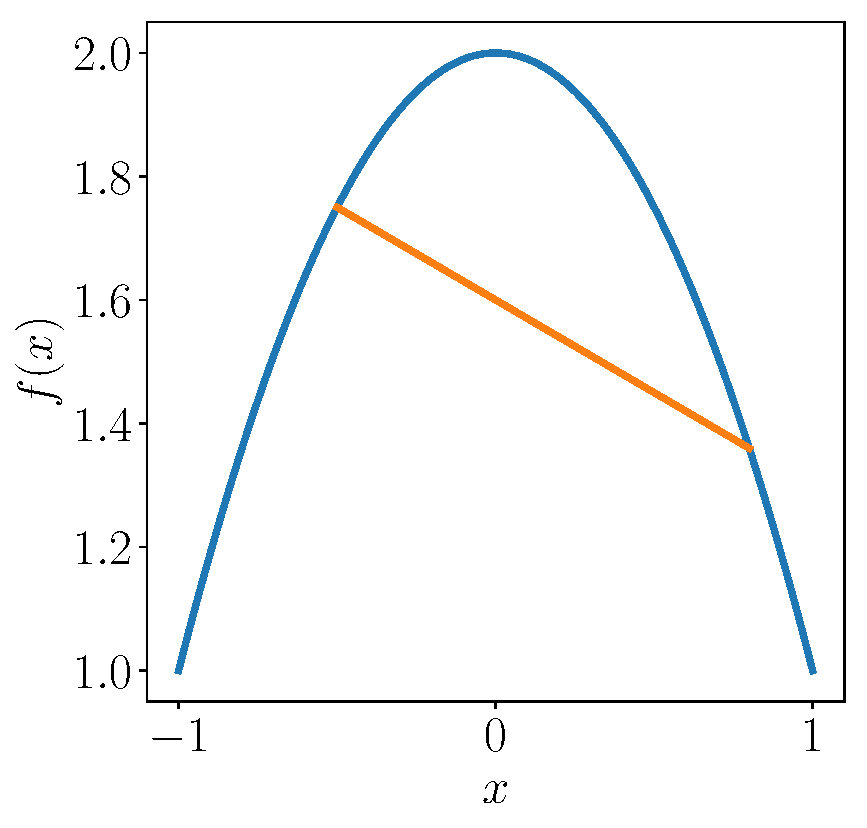
\includegraphics[width=\hsize]{./figures/vi/concave_function}
\end{columns}
\vspace{4mm}
\pause
Logarithms are concave. Therefore:
\begin{align*}
\log \E[g(\vec z)] = \log \int g(\vec z) p(\vec z) d\vec z \geq \int
p(\vec z) \log g(\vec z) d\vec z = \E[\log g(\vec z)]
\end{align*}
\pause
Idea: For estimating the log marginal likelihood, use Jensen's inequality
instead of Monte Carlo.
\end{frame}


\begin{frame}{Deriving the Variational Lower Bound}
  Look at log-marginal likelihood (log-evidence): 
  \begin{align*}
    \log p(\vec x) &= \log \int p(\vec x|\vec z) p(\vec z) d\vec z\\
    \onslide+<2->{&= \log \int p(\vec x|\vec z) p(\vec z) \frac{q(\vec z)}{q(\vec
    z)}d\vec z\\}
    \onslide+<3->{&= \log \int p(\vec x|\vec z) \frac{p(\vec z)}{q(\vec z)} q(\vec z)
    d\vec z\\}
     \onslide+<4->{&= \log\E_q\left[p(\vec x|\vec z)\frac{p(\vec z)}{q(\vec
    z)}\right]\\}
     \onslide+<5->{&\blue{\geq}\E_q\log\left(p(\vec x|\vec z)\frac{p(\vec z)}{q(\vec
    z)}\right)\\}
     \onslide+<6->{&=\E_q[\log p(\vec x|\vec z)] - \E_q\left[\log\left(\frac{q(\vec
    z)}{p(\vec z)}\right)\right]\\}
     \onslide+<7->{&=\E_q[\log p(\vec x|\vec z)]-\KL{q(\vec z)}{p(\vec z)}}
  \end{align*}
\end{frame}



\begin{frame}{What have we gained?}
Marginal likelihood bound\footnote{Also called \emph{negative variational free energy}, or \emph{Evidence Lower BOund} (ELBO).}:
\begin{align}
\lb(q) = \E_q[\log p(\vec x|\vec z)]-\KL{q(\vec z)}{p(\vec z)}
\end{align}

\begin{itemize}
\item Objective function that can be optimised to find $q(\vz)$
\begin{itemize}
\item Terms only include prior and likelihood (can evaluate)
\item Often, integrals \emph{can} be found in closed form!
\end{itemize} \pause
\item Bound allows us to compare approximations! Higher is better.
\begin{itemize}
\item Compare to importance sampling: Two estimates with unknown variances. Don't know which one to believe!
\end{itemize}
\end{itemize}

\pause

\vspace{0.3cm}
With parameterised $q_\mathbf{v}(\vz)$, use gradient-based optimisation to find $\vv$.

\end{frame}




\begin{frame}
  \begin{center}
    A different derivation: \\
    \Large \emph{Minimising the KL}
  \end{center}
\end{frame}





\begin{frame}{What is the measure of similarity?}
\begin{itemize}
\item So far, the justification for VI came from that if $q(\vz) = p(\vz\given\vx)$, then $\lb = \log p(\vx)$.
\item Measure of similarity to $p(\vz\given\vx)$ was defined simply as ``how good a bound'' does the $q(\vz)$ give.
\end{itemize}
\pause

\vspace{0.5cm}
\begin{center}
\large \emph{Can we understand more about the measure of similarity?}
\end{center}
\end{frame}






\begin{frame}{What is the measure of similarity?}
We can find an equation for the measure of similarity by investigating the difference between $\lb$ and $\log p(\vx)$:
\begin{align*}
\log p(\vx) - \lb &= \log p(\vx) - \int q(\vz) \log \frac{p(\vx\given\vz)p(\vz)}{q(\vz)} \calcd{\vz} \\
&= \int q(\vz) \log p(\vx) \calcd{\vz} - \int q(\vz) \log \frac{p(\vx\given\vz)p(\vz)}{q(\vz)} \calcd{\vz} \\
&= \int q(\vz) \log \frac{p(\vx) q(\vz)}{p(\vx\given\vz)p(\vz)} \calcd{\vz} \\
&= \int q(\vz) \log \frac{q(\vz)}{p(\vz\given\vx)} \calcd{\vz} \\
&= \KL{q(\vz)}{p(\vz\given\vx)}
\end{align*}
\pause
\vspace{-0.3cm}
\begin{center}
\Large \emph{VI minimises the KL from the true posterior!}
\end{center}
\end{frame}





% \begin{frame}
%   \begin{center}
%     \Large \emph{Analytic bounds and optimisation}
%   \end{center}
% \end{frame}




% \begin{frame}{Model Class}
% Exact Bayes is intractable, variational inference is tractable.

%   \begin{center}
%   \begin{tikzpicture}
    \node[latent](z) at (-2,0) {$\vec z_n$};
    \node[obs](x) at (0,0) {$\vec x_n$};
    \node[latent](beta) at (-1,1){$\vec\beta$};
    %\edge{z,mu,sigma}{x};
    \edge{z}{x}
    \edge{beta}{x,z}
    \plate {xz} {(x)(z)} {$n=1,\dotsc, N$} ;
    \node[const] at (-4,0) {\small Local variables};
    \node[const] at (-3.9,1) {\small Global variables};
\end{tikzpicture}
%%% Local Variables:
%%% mode: latex
%%% TeX-master: "../lecture_variational_inference"
%%% End:

% \end{center}
%   \begin{itemize}
% \item All unknown parameters are described by random variables
%   \begin{itemize}
%   \item \cemph{Global random variables $\vec\beta$}, which control all
%     the data
%   \item \cemph{Local random variables $\vec z_n$}, which are local to
%     individual data points $\vec x_n$
%   \end{itemize}
%   \pause
% \item Example: Gaussian mixture model
%   \pause
  
%   \begin{itemize}
%   \item Global: means, covariances, weights $\vec\mu_k, \mat\Sigma_k, \pi_k$
%   \item Local: assignments $\vec z_{n}$
%   \end{itemize}
% % \item Generally: global parameters $\beta$, local parameters
% %     (per data point) $z_n$
%   \end{itemize}

% \end{frame}


% \begin{frame}{Complete Conditional}
% \begin{center}
%   \begin{tikzpicture}
    \node[latent](z) at (-2,0) {$\vec z_n$};
    \node[obs](x) at (0,0) {$\vec x_n$};
    \node[latent](beta) at (-1,1){$\vec\beta$};
    %\edge{z,mu,sigma}{x};
    \edge{z}{x}
    \edge{beta}{x,z}
    \plate {xz} {(x)(z)} {$n=1,\dotsc, N$} ;
    \node[const] at (-4,0) {\small Local variables};
    \node[const] at (-3.9,1) {\small Global variables};
\end{tikzpicture}
%%% Local Variables:
%%% mode: latex
%%% TeX-master: "../lecture_variational_inference"
%%% End:

% \end{center}


%   \begin{itemize}
%     \item \emph{Complete conditional:} Conditional of a single latent
%       variable given the observations and all other latent variables
%       \begin{align*}
%         &p(\vec z_n|\vec \beta, \vec x_n)\\
%         &p(\vec \beta|\vec z_{1:N}, \vec x_{1:N})
%       \end{align*}
%       \pause
%       \vspace{-5mm}
%     \item Assume that each \cemph{complete conditional} is a member of
%       the \cemph{exponential family} (Bernoulli, Beta, Gamma,
%       Gaussian, ...)\\
%       \arrow \cemph{Conditionally conjugate models}
%     \end{itemize}
% \end{frame}


% \begin{frame}{Generic Class of Models: Examples}
%     \begin{itemize}
%     \item Bayesian mixture models
%     \item Hidden Markov models
%     \item Factor analysis
%     \item Principal component analysis
%     \item Linear regression
%     \end{itemize}
%   \end{frame}




% \begin{frame}{Example: Gaussian Mixture Model}
% \begin{center}
%   \begin{tikzpicture}
    \node[latent](z) at (-2,0) {$\vec z_n$};
    \node[obs](x) at (0,0) {$\vec x_n$};
    \node[latent](beta) at (-1,1){$\vec\beta$};
    %\edge{z,mu,sigma}{x};
    \edge{z}{x}
    \edge{beta}{x,z}
    \plate {xz} {(x)(z)} {$n=1,\dotsc, N$} ;
    \node[const] at (-4,0) {\small Local variables};
    \node[const] at (-3.9,1) {\small Global variables};
\end{tikzpicture}
%%% Local Variables:
%%% mode: latex
%%% TeX-master: "../lecture_variational_inference"
%%% End:

% \end{center}
% \begin{align*}
% \vec \beta &= \left\{\vmu_k, \mat \Sigma_k, \pi_k\right\}_{k=1}^K \\
% p(\vmu_k, \mat \Sigma_k) &= \NormDist{\vmu_k; 0, \mat \Sigma_k}\mathrm{Wi}\inv\left(\Sigma_k ; \mat \Sigma_0, \nu_0 \right) && \text{Normal-Wishart}\\
% p(\vec \pi) &= \mathrm{Dir}\left(\vec \pi ; \vec \alpha_0\right) && \text{Dirichlet}\\
% P(z_n = k\given \vec\pi) &= \pi_k && \text{Categorical} \\
% p(\vx_n\given z_n = k, \vec \beta) &= \NormDist{\vx_n; \vmu_k, \mat\Sigma_k}
% \end{align*}
% \end{frame}


% \begin{frame}{Example: Gaussian Mixture Model}
% Gaussian Mixture Model is conditionally conjugate.
% \begin{align}
% p(z_n = k \given \vec\beta, \vx_n) &= \frac{\NormDist{\vx_n; \vmu_k, \mat\Sigma_k}\pi_k}{\sum_{k'=1}^K \NormDist{\vx_n; \vmu_{k'}, \mat\Sigma_{k'}}\pi_{k'}} && \text{Categorical} \\
% p(\vec\beta\given \{z_n, \vx_n\}_{n=1}^N) &= \mathrm{Dir}\left(\vec\alpha_0 + \vec n\right) \nonumber \\
% & \qquad \prod_{k=1}^K \NormDist{\vmu_k; \vm_k, \frac{1}{1 + N}\mat\Sigma_k} \nonumber \\
% & \qquad \mathrm{Wi}\inv\left(
% \Sigma_k; \mat S_k, \nu_k\right) \\
% \vm_k = \frac{N}{1 + N}\bar{\vx}_k \,, &\mat S_k = \mat S_0 + \bar{\mat S}_k \,, \nu_N = \nu_0 + N
% \end{align}
% \pause
% (See Murphy \S 4.6)
% \end{frame}



% \begin{frame}{VI for Conditionally Conjugate Models}
% We will discuss a \emph{general} variational procedure for \emph{conditionally conjugate models}, using the Gaussian Mixture Model as an example.

% \pause

% \vspace{0.5cm}

% Procedure:
% \begin{enumerate}
% \item Remember our objective (ELBO)
% \item Choose a family of approximating distributions, such that we can compute objective
% \item Optimise objective w.r.t.~approximating distribution
% \end{enumerate}
% \end{frame}





% \begin{frame}{VI for Conditionally Conjugate Models}
%   Single assumption, fully factorised (mean field) approximation:
%   \begin{align*}
%     q_{\vec v}(\vec \beta, \vec z) = q_{\vec\lambda}(\vec \beta) \prod_{n=1}^N q_{\vec\phi_n}(\vec
%     z_n)    \,, \quad \vec\nu = \{\vec\lambda,
%     \vec\phi_1,\dotsc, \vec\phi_N\}
%   \end{align*}

%   \vspace{0.5cm}

%   From this assumption, we can derive the \emph{optimal factor} given all other factors are fixed, i.e.~we find
%   \begin{align*}
%     q^*(\vz_n) = \argmax_{q(\vz_n) \in \mathcal{Q}} \lb(q_{\vec v}(\vec\beta, \vec\vz))
%   \end{align*}
%   where $\mathcal{Q}$ is the space of all possible densities.
% \end{frame}


% \begin{frame}{Optimizing in Turn}
%   \begin{itemize}
%   \item Independent latent variables: \colchar{$q(\vec z) = \prod_n
%     q(\vec z_n|\vec\phi_n)=\prod_nq_n(\vec z_n)$}{blue}\newline
%     \arrow Optimize variational
%     parameters in turn
%     \begin{align*}
%       \onslide+<2->{\text{ELBO} &=\E_q\left[\log \left(p(\vec x|\vec z)
%                                   \frac{p(\vec z)}{q(\vec z)}\right)\right]
%                                   }
%       %=\E_q\left[\log \frac{p(\vec x, \vec z)}{q(\vec z)}\right] \\
% \onslide+<3->{
%       = \E_q[\orange{\log p(\vec x, \vec z)} \blue{- \log q(\vec z)}]\\
%       }
%       \onslide+<4->{
%       &=\orange{ \E_{q_n}\Big[\underbrace{\E_{i\neq n}[\log p(\vec x, \vec
%         z)]}_{=:\hat p(\vec x, \vec z_n)}\Big]} \blue{-
%         \E_{q_n}[\log q_n(\vec z_n)] - \sum_{i\neq n}\E_{q_i}[\log q_i(\vec
%         z_i)]}\\
%       }
%       \onslide+<5->{
%       &=\orange{\E_{q_n}[\hat p(\vec x, \vec z_n)]}\blue{ - \E_{q_n}[\log q_n(\vec z_n)]
%       - \sum_{i\neq n}\E_{q_i}[\log q_i(\vec
%         z_i)]}
%         }
%     \end{align*}
%     \onslide+<6->{
%     \item Fix $q_{i\neq n}$ and optimize factor $q_n$:
%     }
%  \onslide+<7->{
%     \begin{align*}
%       \text{ELBO}(q_n) & = \E_{q_n}[\hat p(\vec x, \vec z_n)] - \E_{q_n}[\log
%                   q_n(\vec z_n)] + \text{const}\\
%       \onslide+<8->{
%                        &= \E_{q_n}\left[\log \frac{\exp(\hat p(\vec x, \vec
%         z_n))}{q_n(\vec z_n)}\right] = -\KL{q_n(\vec z_n)}{\exp(\hat p(\vec x, \vec
%                          z_n))}
%                          }
%     \end{align*}
%     }
%   \end{itemize}
% \end{frame}
% %%%%%%%%%%%%%%%%%%%%%%%%%%%%%%%%%%%%%%%%%%%%%
% \begin{frame}{Optimal Factors}
%   \begin{align*}
%       \text{ELBO}(q_n) &=  -\KL{q_n(\vec z_n)}{\exp(\hat p(\vec x, \vec
%         z_n))}
%     \end{align*}
%   \begin{itemize}[<+->]
%   \item Maximizing the ELBO w.r.t. $q_n$ is equivalent to minimizing $\KL{q_n(\vec z_n)}{\exp(\hat p(\vec x, \vec
%       z_n))}$
%       $$
%       \arrow~\colchar{$\log q_n^*(\vec z_n) = \hat p(\vec x, \vec z_n) =
%       \E_{q_{i\neq n}} [\log p(\vec x, \vec z)] + \text{const}$}{blue}
%       $$
%     \item
%       Get the optimal factor $q_n^*$ by
%       \begin{enumerate}
%         \item Writing down the log-joint distribution of all latent
%           and observed variables $\log p(\vec x, \vec z)$
%          \item Computing the expectation w.r.t. all other random variables
%       \end{enumerate}
%     \end{itemize}
% \end{frame}


% \begin{frame}{Mean-Field VI for Conditionally Conjugate Models}
%   \begin{center}
%     \scalebox{0.8}{\begin{tikzpicture}
    \node[const](phi) at (-2,0) {\fixgmfont{$\vec\phi_n$}};
    \node[latent](z) at (0,0) {$\vec z_n$};
    \node[latent](beta) at (0,1){$\vec\beta$};
    \node[const](lambda) at (-2,1) {\fixgmfont{$\vec\lambda$}};
    %\edge{z,mu,sigma}{x};
    \edge{lambda}{beta}
    \edge{phi}{z}
    \plate {zphi} {(z)(phi)} {$n=1,\dotsc, N$} ;
\end{tikzpicture}
%%% Local Variables:
%%% mode: latex
%%% TeX-master: "../lecture_variational_inference"
%%% End:
}
%   \end{center}
%   \begin{itemize}[<+->]
%   \item \cemph{Optimal factors} (see Bishop (2006)\nocite{Bishop2006} or
%     Ghahramani \& Beal (2001)\nocite{Ghahramani2001, Beal2003}):
%     \begin{align*}
%       % q^*(\vec\beta|\vec\lambda)&~\propto~\exp\left(\E_{\vec\phi_{1:N}}[\log
%       %   p(\vec x, \vec z)]\right)\\
%       % q^*(\vec z_n|\vec\phi_n) &~\propto~\exp\left(\E_{\vec\lambda}[\log p(\vec
%       %   x_n, \vec\beta)]\right)
%                                    q^*(\vec\beta|\vec\lambda)&~\propto~\exp\left(\E_{\vec z}[\log
%                                                                p(\vec x, \vec z, \vec\beta)]\right)\\
%       q^*(\vec z_n|\vec\phi_n) &~\propto~\exp\left(\E_{\vec\beta}[\log p(\vec
%                                  x_n, \vec z_n, \vec\beta)]\right)
%     \end{align*}
%   \item Update one term at a time \arrow \cemph{Coordinate ascent}
%   \item No closed-form solution (see EM algorithm)
%   \item Iteratively optimize each parameter until we reach a local
%     optimum (convergence guaranteed)
%   \end{itemize}
% \end{frame}


% \begin{frame}{Mean-Field VI: Algorithm}
%   \begin{enumerate}
%   \item Input: data $\vec x$, model $p(\vec\beta, \vec z, \vec x)$
%   \item Initialize global variational parameters $\vec\lambda$ randomly
%   \item While ELBO has not converged, repeat:
%     \begin{enumerate}
%     \item For each data point $\vec x_n$
%       \begin{enumerate}
%       \item Update local variational parameters $\vec\phi_n$
%       \end{enumerate}
%     \item Update global variational parameters $\vec\lambda$
%     \end{enumerate}
%   \end{enumerate}
% \end{frame}



% \begin{frame}{Example: Gaussian Mixture Models}
% See Bishop \S 10.2, or Murphy \S 21.6 for full derivation.

% \vspace{0.5cm}

% What do we gain compared to Maximum Likelihood? \pause
% \begin{itemize}
% \item Approximate posterior over $\{\vmu_k, \mat \Sigma_k\}$ prevents catastrophic overfitting (board) \pause
% \item ELBO as an approximation to the marginal likelihood \\
% \arrow Tells us how many components to use.
% \end{itemize}
% \end{frame}







\begin{frame}
  \begin{center}
    \Large \emph{Properties of Variational Inference}
  \end{center}
\end{frame}




\begin{frame}{Properties of the KL divergence}
The KL divergence is a \emph{measure of difference} between probability distributions.
\begin{align}
\mathrm{KL} = \KL{q(\vz)}{p(\vz)} = \int q(\vz) \log \frac{q(\vz)}{p(\vz)} \calcd{\vz}
\end{align}
\vspace{-0.8cm}
\begin{itemize}
\item $\mathrm{KL} \geq 0$ \pause
\item $\mathrm{KL} = 0$ iff $q(\vz) = p(\vz)$ \pause
\item Related to information theory and code lengths \pause
\item Related to decision theory and betting returns \pause
\item Intuitively:
\begin{itemize}
\item Strong penalty for $q(\vz)$ for placing mass where $p(\vz)$ doesn't
\item Weak penalty for $q(\vz)$ for placing too much mass compared to $p(\vz)$
\end{itemize}
\end{itemize}
\end{frame}


\begin{frame}{Example: Gaussian KL divergence}
  \begin{center}
    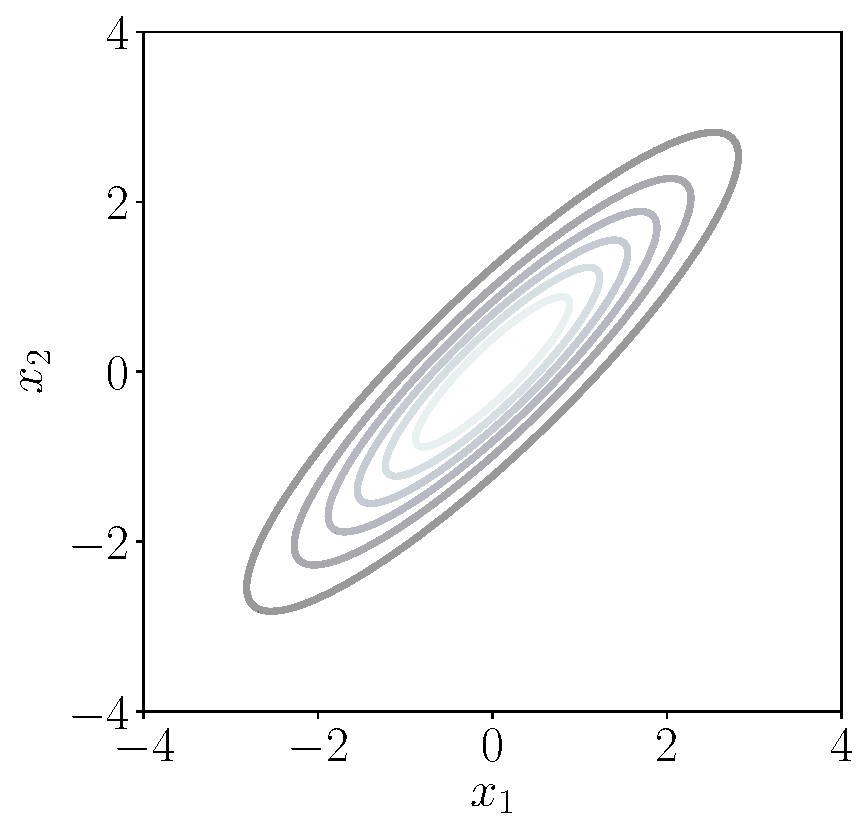
\includegraphics[width=0.4\hsize]{./figures/vi/mean_field_vi_original}%
    \hspace{5mm}
    \onslide+<2->{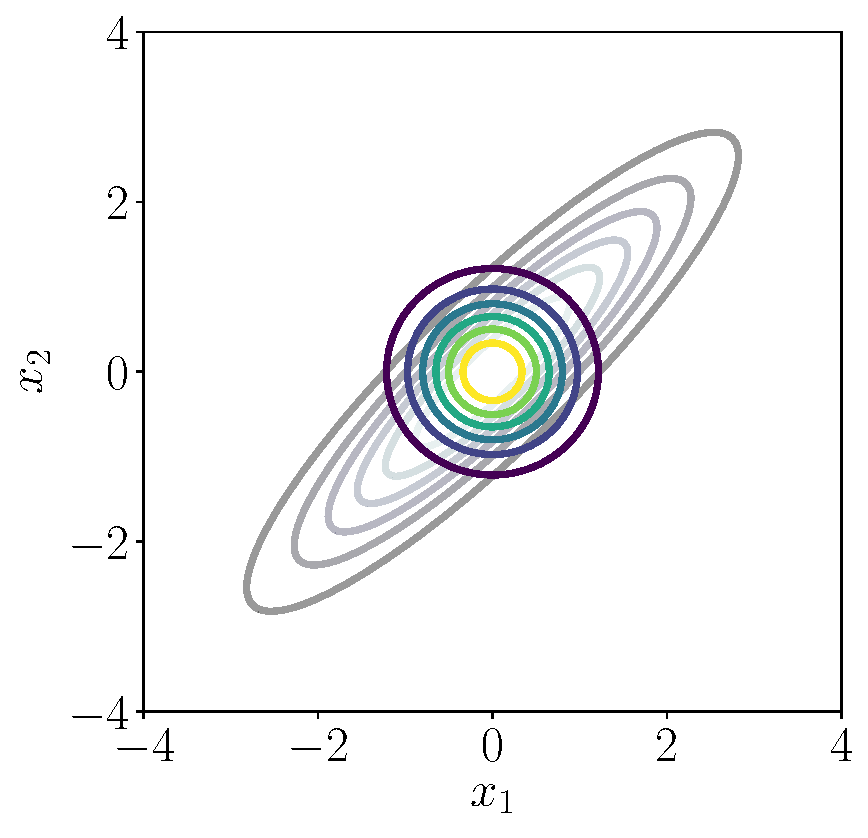
\includegraphics[width=0.4\hsize]{./figures/vi/mean_field_vi_approx}}%
  \end{center}
  \vspace{-0.6cm}
  \begin{align*}
    &\KL{\NormDist{\vx; \vmu_0, \Sigma_0}}{\NormDist{\vx; \vmu_1, \Sigma_1}} = \\
    & \qquad \frac{1}{2}\left[\Tr\left(\Sigma_1\inv\Sigma_0\right) + (\vmu_1 - \vmu_0)\transpose\Sigma_1\inv(\vmu_1 - \vmu_0)) - D + \log \frac{\det \Sigma_1}{\det \Sigma_0} \right]
  \end{align*}
  \vspace{-0.6cm}
  \begin{itemize}
  \item $\Sigma_0\to \mathbf{0} \qquad \implies \qquad \mathrm{KL} \to \infty$
  \end{itemize}
\end{frame}


\begin{frame}{Approximating Distributions}
  \begin{center}
    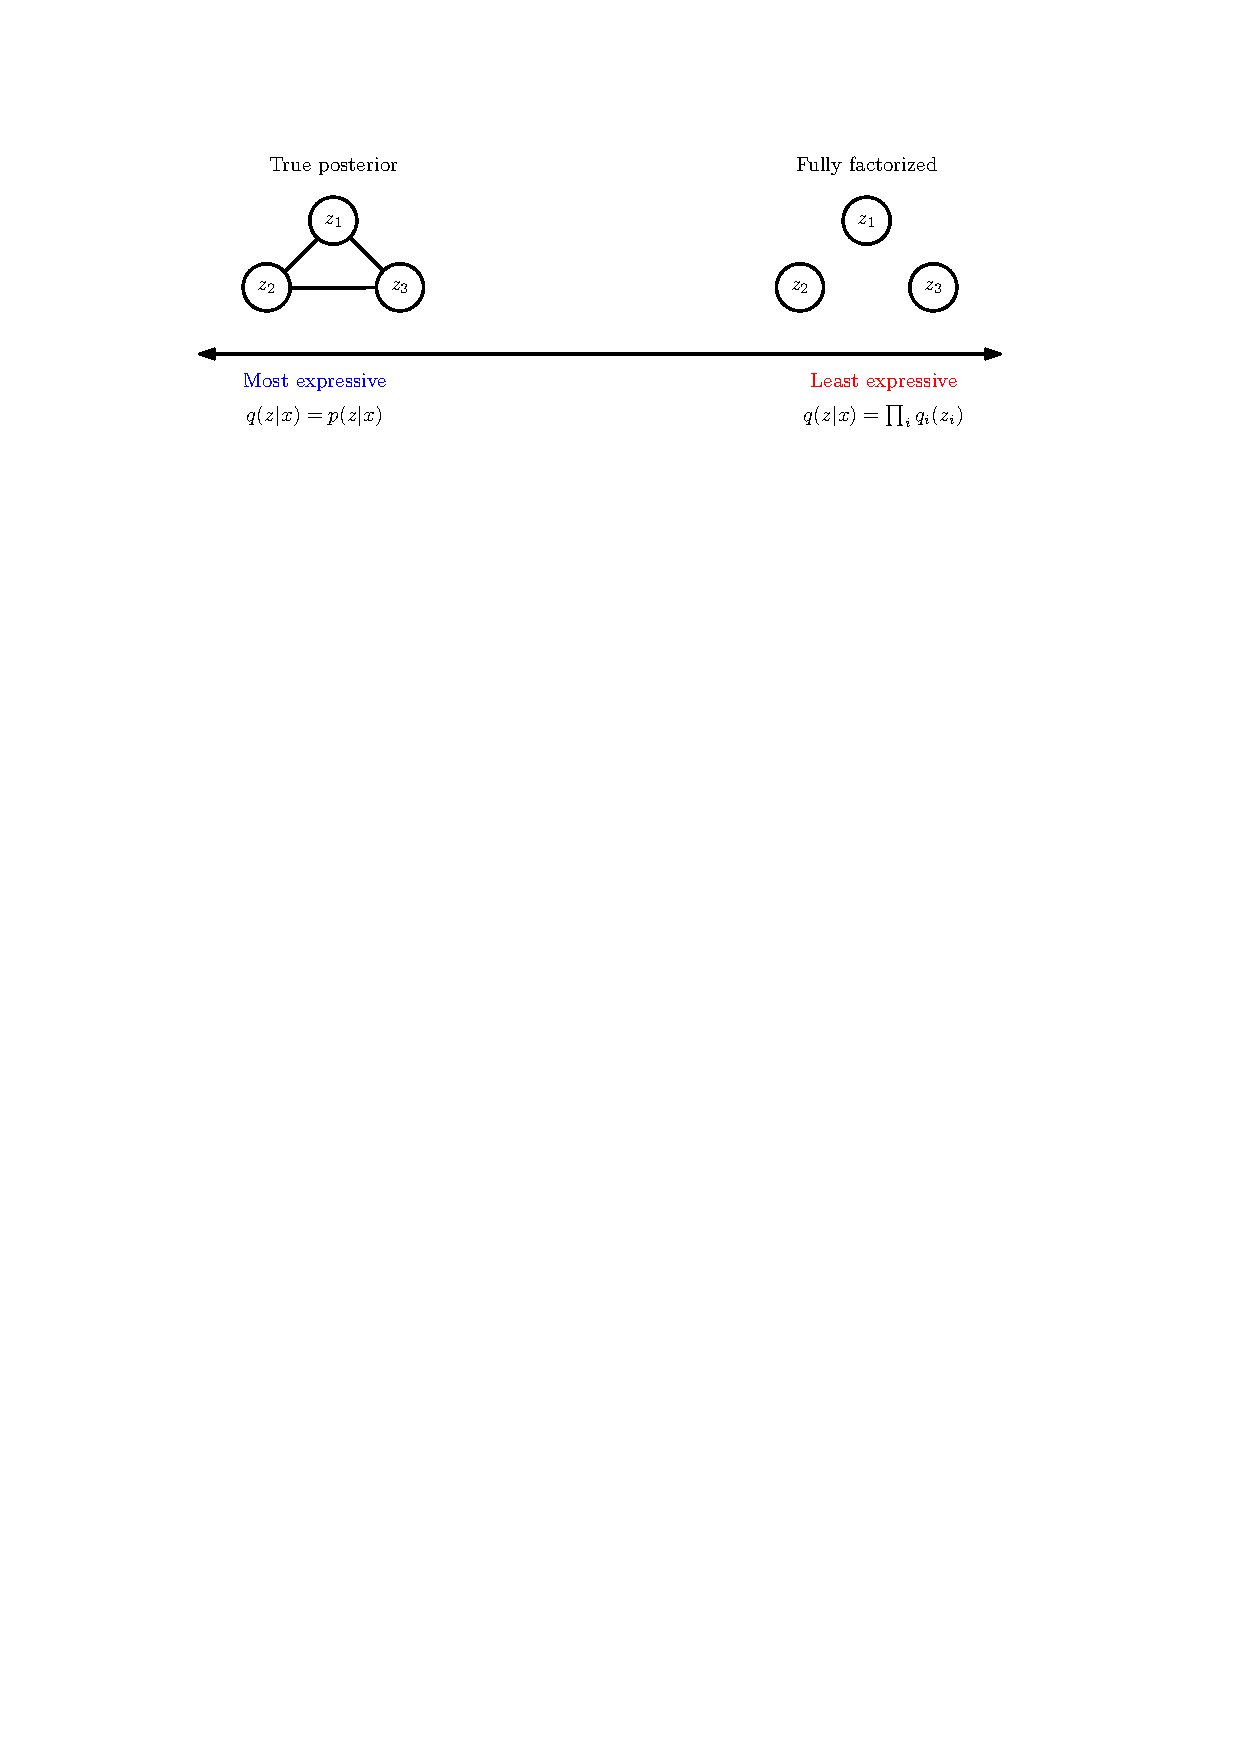
\includegraphics[width=0.85\hsize]{./figures/vi/families_of_q}
  \end{center}

  \pause
  Trade-off
  \begin{itemize}
    \item More expressive gets closer to the true posterior
    \item Less expressive is easier to handle
    \item Expressive distributions may not allow integrals in ELBO to be computed
  \end{itemize}
  % \begin{itemize}
  % \item Specifying the class of posteriors is closely related to
  %   specifying a model of the data\\
  %   \arrow We have a lot of flexibility \pause
  % \item Generally:
  %   \begin{itemize}
  %   \item Build \cemph{expressive class of posteriors} (no
  %     overfitting problems)
  %   \item Maintain \cemph{computational efficiency} \arrow \cemph{Scalability}
  %   \end{itemize}
  % \end{itemize}
\end{frame}



\begin{frame}{Mean-Field Approximation: Limitation}
  \begin{center}
    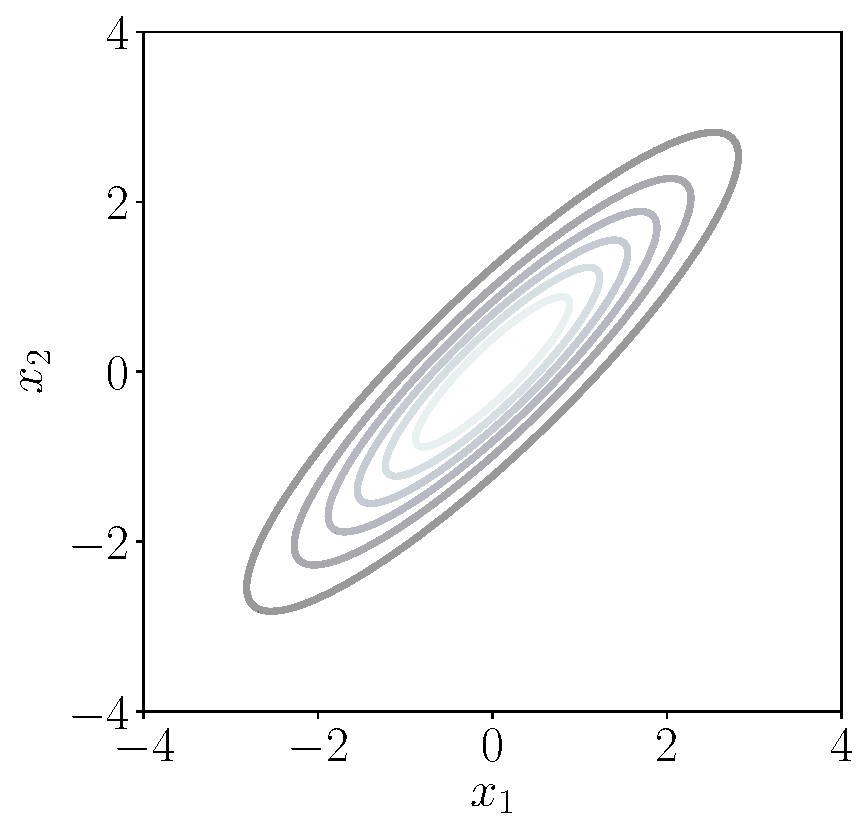
\includegraphics[width=0.4\hsize]{./figures/vi/mean_field_vi_original}%
    \hspace{5mm}
    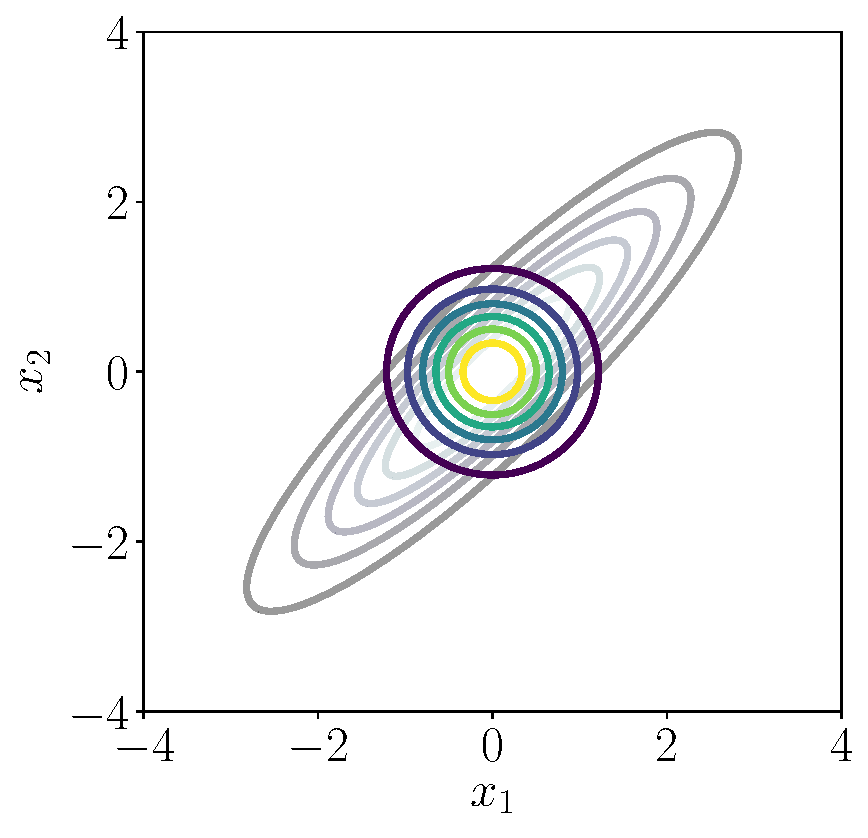
\includegraphics[width=0.4\hsize]{./figures/vi/mean_field_vi_approx}
  \end{center}

  \begin{itemize}
    \item Mean-field VI to approximate a correlated Gaussian with a
      factorized Gaussian
    \item Generally, mean-field VI tends to yield an approximation
      that is \calert{too compact} \arrow Need better classes of
      posterior approximations
  \end{itemize}
\end{frame}




\begin{frame}{Interpretation of terms}
  \begin{align*}
    \log p(\vec x) &\geq
    % q(\vec x)\log \left(p(\vec x | \vec z)
    % \frac{p(\vec z)}{q(\vec z)}\right)d\vec z\\
    % &= \int q(\vec z) \log p(\vec x|\vec z)d\vec z -\int q(\vec
    % z)\log\frac{q(\vec z)}{p(\vec z)}d\vec z\\
    % &= \orange{\E_q[\log p(\vec x|\vec z)]} - \blue{\E_q\left[\log\frac{q(\vec
    % z)}{p(\vec z)}\right]} \\
    \orange{\E_q[\log p(\vec x|\vec z)]} - \blue{\KL{q(\vec z)}{p(\vec z)}}=:\text{ELBO}
  \end{align*} \pause

  \begin{itemize}
  \vspace{-5mm}
  \item \orange{Data-fit term} (expected log-likelihood): Measures how
    well samples from $q(\vec z)$ explain the data (``reconstruction cost''). \\
    \arrow Place $q$'s mass on the MAP estimate. 
  \item \blue{Regularizer:} Variational posterior $q(\vec z)$
    should not differ much from the prior $p(\vec z)$
  \end{itemize}
\end{frame}







\begin{frame}{Alternative form of ELBO}
\begin{align*}
\lb(q_\vv) &= \int q_\vv(\vz) \log p(\vx\given\vz) \calcd{\vz} &&- \underbrace{\int q_\vv(\vz) \log \frac{q_\vv(\vz)}{p(\vz)}}_{\text{KL}} \calcd{\vz} \\
&= \int q_\vv(\vz) \log p(\vx\given\vz) p(\vz) \calcd\vz &&-\int q_\vv(\vz) \log q_\vv(\vz) \calcd\vz \\
&= \int q_\vv(\vz) \log p(\vx\given\vz) p(\vz) \calcd\vz &&+ \mathcal{H}(q_\vv(\vz))
\end{align*}
\end{frame}



\begin{frame}{Comparison to MAP}
\begin{align}
\lb(q_\vv) &= \int q_\vv(\vz) \log p(\vx\given\vz)p(\vz) \calcd{\vz} &&+ \mathcal{H}(q_\vv(\vz)) \\
L_{\text{MAP}}(\vz) &= \log p(\vx|\vz) + \log p(\vz) &&
\end{align}

\pause

\begin{itemize}
  \item Fit the data like MAP
  \item but also be as \emph{uncertain} as possible (entropy)
\end{itemize}
\end{frame}


\begin{frame}{Properties of the differential entropy}
\begin{align}
\mathcal{H}[q(\vz)] = - \int q(\vz) \log q(\vz) \calcd{\vz}
\end{align}
\begin{itemize}
  \item Generalises entropy to continuous variables
  \item Limit of: Entropy of quantised $q(\vz)$ minus uniform distribution
  \item Can be negative! (i.e.~more certain than a uniform)
\end{itemize}
\end{frame}




\begin{frame}{Summary}
\begin{itemize}
\item Variational turns inference into optimisation
\item Two ways to derive:
\begin{itemize}
\item We minimise the KL divergence to the posterior
\item Lower bound marginal likelihood with Jensen's inequality
\end{itemize}
\item Constrained approximation families (e.g.~mean-field) tend to underestimate uncertainty
\end{itemize}

\vspace{0.4cm}

Next time:
\begin{itemize}
\item How to compute ELBOs
\item How to optimise ELBOs
\end{itemize}
\end{frame}














% \begin{frame}{Conditionally conjugate models}
% For \emph{conditionally conjugate models}, we have
% \begin{itemize}
% \item a way to find the \emph{optimal form} of each approximation term,
% \item closed-form ELBOs,
% \item a specialised way of optimising terms without gradients.
% \end{itemize}

% \pause
% \vspace{1.0cm}

% Next time...
% \end{frame}


%%%%%%%%%%%%%%%%%%%%%%%%%%%%%%%%%%%%%%%%%%%%%%%
% \section{Mean-Field Variational Inference}


% %%%%%%%%%%%%%%%%%%%%%%%%%
% \begin{frame}{Mean-Field Approximation}
% \begin{center}
%     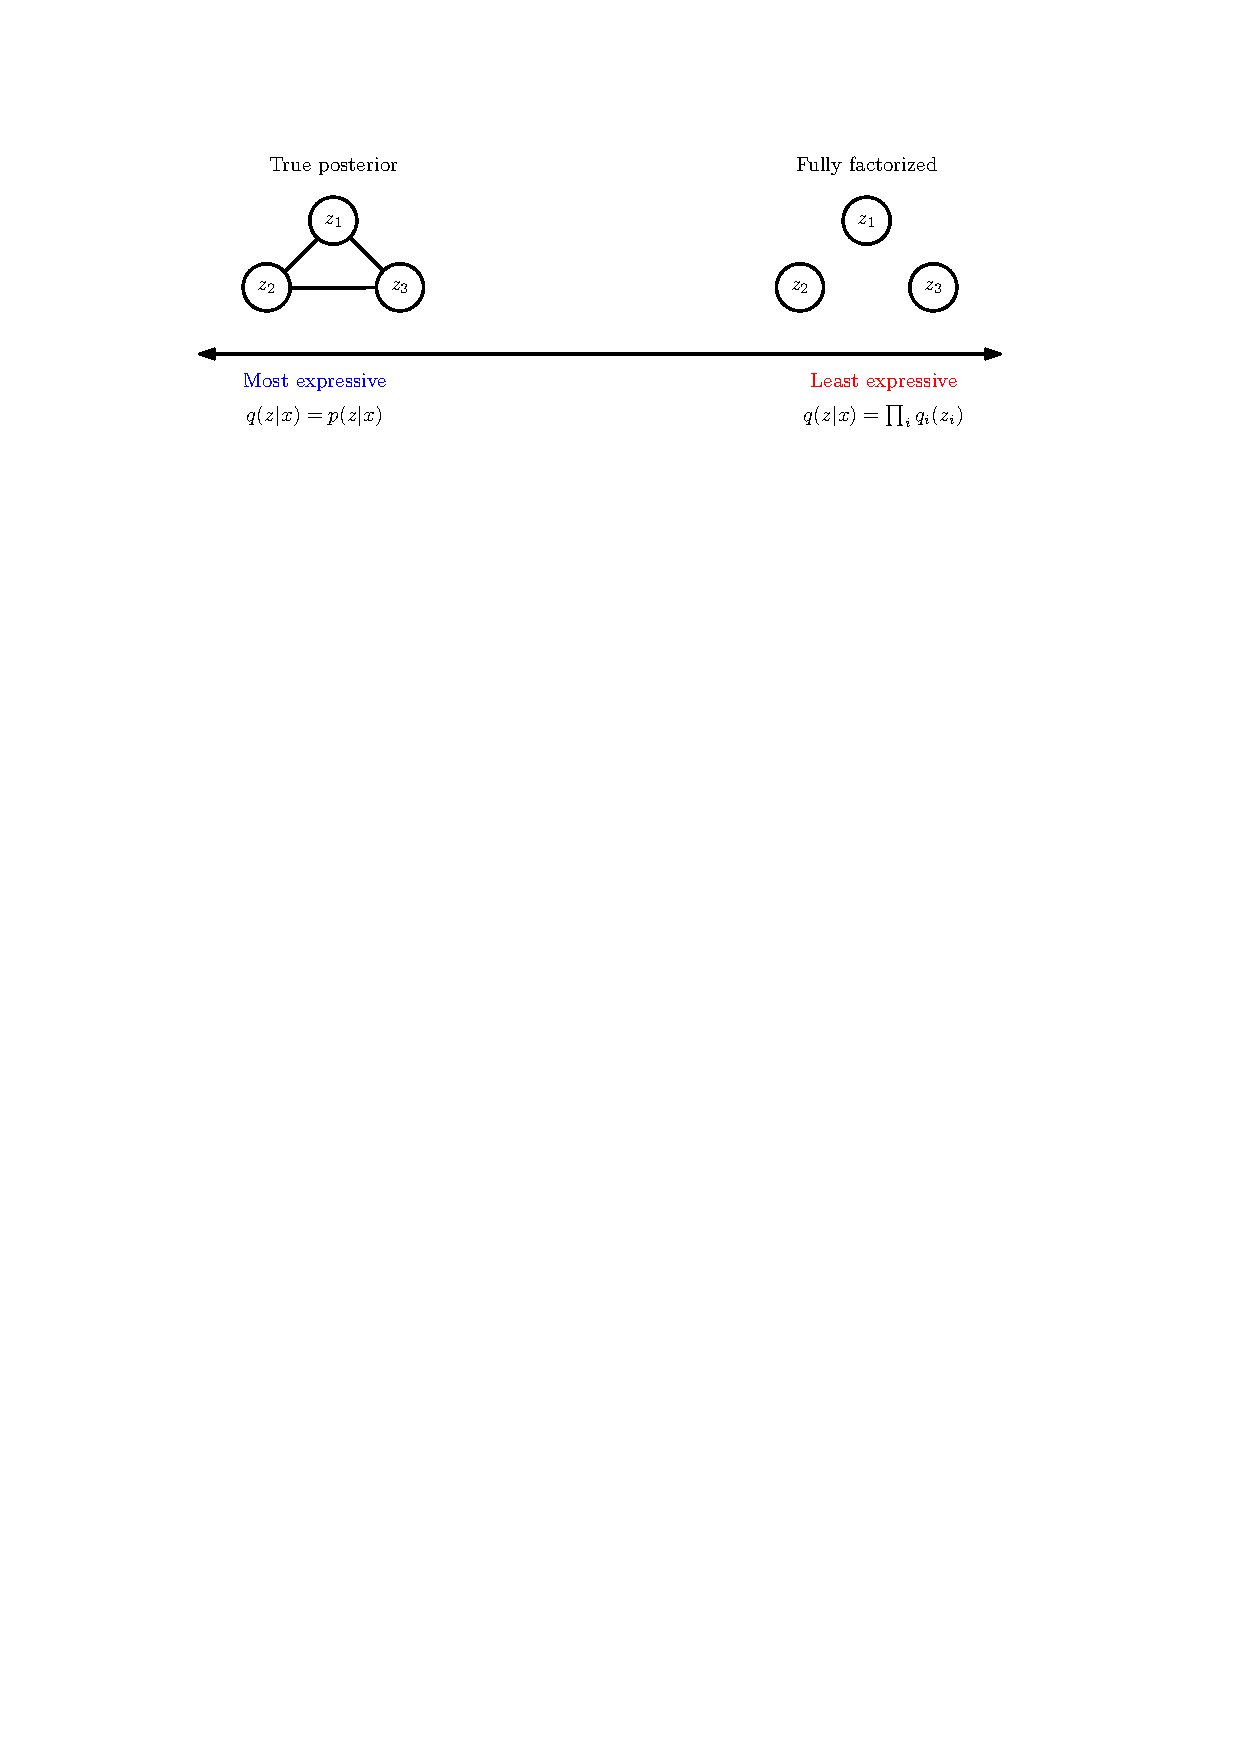
\includegraphics[width=0.85\hsize]{./figures/vi/families_of_q}
%   \end{center}
%   \begin{itemize}
%   \item Assume conditionally conjugate model
%   \item \cemph{Fully factorized (mean field)} approximation:
%     \begin{columns}
%       \column{0.7\hsize}
%     \begin{align*}
%       q(\vec \beta, \vec z|\vec\nu) = q(\vec \beta|\vec\lambda) \prod_{n=1}^N q(\vec
%       z_n|\vec\phi_n) 
%     \end{align*}
%     \column{0.4\hsize}
%     \begin{center}
%   \scalebox{0.8}{\begin{tikzpicture}
    \node[const](phi) at (-2,0) {\fixgmfont{$\vec\phi_n$}};
    \node[latent](z) at (0,0) {$\vec z_n$};
    \node[latent](beta) at (0,1){$\vec\beta$};
    \node[const](lambda) at (-2,1) {\fixgmfont{$\vec\lambda$}};
    %\edge{z,mu,sigma}{x};
    \edge{lambda}{beta}
    \edge{phi}{z}
    \plate {zphi} {(z)(phi)} {$n=1,\dotsc, N$} ;
\end{tikzpicture}
%%% Local Variables:
%%% mode: latex
%%% TeX-master: "../lecture_variational_inference"
%%% End:
}
% \end{center}
%   \end{columns}
% \end{itemize} 
% \end{frame}

% %%%%%%%%%%%%%%%%%%%%%%%%%
% \begin{frame}{Fully Factorized Distribution}
%   \begin{itemize}[<+->]
%   \item \cemph{Fully factorized (mean field)} approximation:
%     \begin{align*}
%       q(\vec \beta, \vec z|\vec\nu) = q(\vec \beta|\vec\lambda) \prod_{n=1}^N q(\vec
%       z_n|\vec\phi_n)    \,, \quad \vec\nu = \{\vec\lambda,
%                                  \vec\phi_1,\dotsc, \vec\phi_N\}
%     \end{align*}
%     %
%       \item All latent variables are \cemph{independent} and governed by their \cemph{own
%       variational parameters}
%     \item Assume each factor is in the same exponential family as the model's
%       complete conditional
%     \item \calert{The $q$-factors do not depend on the data}
%     \item \cemph{ELBO connects this family to the data}
%     \item Maximize the ELBO w.r.t. variational parameters $\vec\nu$
%   \end{itemize} 
% \end{frame}

% %%%%%%%%%%%%%%%%%%%%%%%%%%%%%%%%%%%%%%%%%%%%%
% \begin{frame}{Optimizing in Turn}
%   \begin{itemize}
%   \item Independent latent variables: \colchar{$q(\vec z) = \prod_n
%     q(\vec z_n|\vec\phi_n)=\prod_nq_n(\vec z_n)$}{blue}\newline
%     \arrow Optimize variational
%     parameters in turn
%     \begin{align*}
%       \onslide+<2->{\text{ELBO} &=\E_q\left[\log \left(p(\vec x|\vec z)
%                                   \frac{p(\vec z)}{q(\vec z)}\right)\right]
%                                   }
%       %=\E_q\left[\log \frac{p(\vec x, \vec z)}{q(\vec z)}\right] \\
% \onslide+<3->{
%       = \E_q[\orange{\log p(\vec x, \vec z)} \blue{- \log q(\vec z)}]\\
%       }
%       \onslide+<4->{
%       &=\orange{ \E_{q_n}\Big[\underbrace{\E_{i\neq n}[\log p(\vec x, \vec
%         z)]}_{=:\hat p(\vec x, \vec z_n)}\Big]} \blue{-
%         \E_{q_n}[\log q_n(\vec z_n)] - \sum_{i\neq n}\E_{q_i}[\log q_i(\vec
%         z_i)]}\\
%       }
%       \onslide+<5->{
%       &=\orange{\E_{q_n}[\hat p(\vec x, \vec z_n)]}\blue{ - \E_{q_n}[\log q_n(\vec z_n)]
%       - \sum_{i\neq n}\E_{q_i}[\log q_i(\vec
%         z_i)]}
%         }
%     \end{align*}
%     \onslide+<6->{
%     \item Fix $q_{i\neq n}$ and optimize factor $q_n$:
%     }
%  \onslide+<7->{
%     \begin{align*}
%       \text{ELBO}(q_n) & = \E_{q_n}[\hat p(\vec x, \vec z_n)] - \E_{q_n}[\log
%                   q_n(\vec z_n)] + \text{const}\\
%       \onslide+<8->{
%                        &= \E_{q_n}\left[\log \frac{\exp(\hat p(\vec x, \vec
%         z_n))}{q_n(\vec z_n)}\right] = -\KL{q_n(\vec z_n)}{\exp(\hat p(\vec x, \vec
%                          z_n))}
%                          }
%     \end{align*}
%     }
%   \end{itemize}
% \end{frame}
% %%%%%%%%%%%%%%%%%%%%%%%%%%%%%%%%%%%%%%%%%%%%%
% \begin{frame}{Optimal Factors}
%   \begin{align*}
%       \text{ELBO}(q_n) &=  -\KL{q_n(\vec z_n)}{\exp(\hat p(\vec x, \vec
%         z_n))}
%     \end{align*}
%   \begin{itemize}[<+->]
%   \item Maximizing the ELBO w.r.t. $q_n$ is equivalent to minimizing $\KL{q_n(\vec z_n)}{\exp(\hat p(\vec x, \vec
%       z_n))}$
%       $$
%       \arrow~\colchar{$\log q_n^*(\vec z_n) = \hat p(\vec x, \vec z_n) =
%       \E_{q_{i\neq n}} [\log p(\vec x, \vec z)] + \text{const}$}{blue}
%       $$
%     \item
%       Get the optimal factor $q_n^*$ by
%       \begin{enumerate}
%         \item Writing down the log-joint distribution of all latent
%           and observed variables $\log p(\vec x, \vec z)$
%          \item Computing the expectation w.r.t. all other random variables
%       \end{enumerate}
%     \end{itemize}
% \end{frame}

% %%%%%%%%%%%%%%%%%%%%%%%%%%%%%%%%%%%%%%%%%%%%% 
% \begin{frame}{Mean-Field Approximation for Conditionally Conjugate Models}
%  \begin{center}
%   \scalebox{0.8}{\begin{tikzpicture}
    \node[const](phi) at (-2,0) {\fixgmfont{$\vec\phi_n$}};
    \node[latent](z) at (0,0) {$\vec z_n$};
    \node[latent](beta) at (0,1){$\vec\beta$};
    \node[const](lambda) at (-2,1) {\fixgmfont{$\vec\lambda$}};
    %\edge{z,mu,sigma}{x};
    \edge{lambda}{beta}
    \edge{phi}{z}
    \plate {zphi} {(z)(phi)} {$n=1,\dotsc, N$} ;
\end{tikzpicture}
%%% Local Variables:
%%% mode: latex
%%% TeX-master: "../lecture_variational_inference"
%%% End:
}
% \end{center}
%   \begin{itemize}[<+->]
%   \item \cemph{Optimal factors} (see Bishop (2006)\nocite{Bishop2006} or
%     Ghahramani \& Beal (2001)\nocite{Ghahramani2001, Beal2003}):
%     \begin{align*}
%       % q^*(\vec\beta|\vec\lambda)&~\propto~\exp\left(\E_{\vec\phi_{1:N}}[\log
%       % p(\vec x, \vec z)]\right)\\
%       % q^*(\vec z_n|\vec\phi_n) &~\propto~\exp\left(\E_{\vec\lambda}[\log p(\vec
%       % x_n, \vec\beta)]\right)
% q^*(\vec\beta|\vec\lambda)&~\propto~\exp\left(\E_{\vec z}[\log
%       p(\vec x, \vec z, \vec\beta)]\right)\\
%       q^*(\vec z_n|\vec\phi_n) &~\propto~\exp\left(\E_{\vec\beta}[\log p(\vec
%       x_n, \vec z_n, \vec\beta)]\right)
%     \end{align*}
%   \item Update one term at a time \arrow \cemph{Coordinate ascent}
%     \item No closed-form solution (see EM algorithm)
%     \item Iteratively optimize each parameter until we reach a local
%       optimum (convergence guaranteed)
%     \end{itemize}
%   \end{frame}
% %%%%%%%%%%%%%%%%%%%%%%%%%%%%%%%%%%%%%%%%%%%%%
%   \begin{frame}{Mean-Field Approximation: Algorithm}
% \begin{enumerate}
% \item Input: data $\vec x$, model $p(\vec\beta, \vec z, \vec x)$
% \item Initialize global variational parameters $\vec\lambda$ randomly
% \item While ELBO has not converged, repeat:
%   \begin{enumerate}
%   \item For each data point $\vec x_n$
%     \begin{enumerate}
%     \item Update local variational parameters $\vec\phi_n$
%     \end{enumerate}
% \item Update global variational parameters $\vec\lambda$
% \end{enumerate}
% \end{enumerate}
% \end{frame}


% %%%%%%%%%%%%%%%%%%%%%%%%%%%%%%%%%%%%%%%%%%%%%

% \begin{frame}{Mean-Field Approximation: Limitation}
%   \begin{center}
%     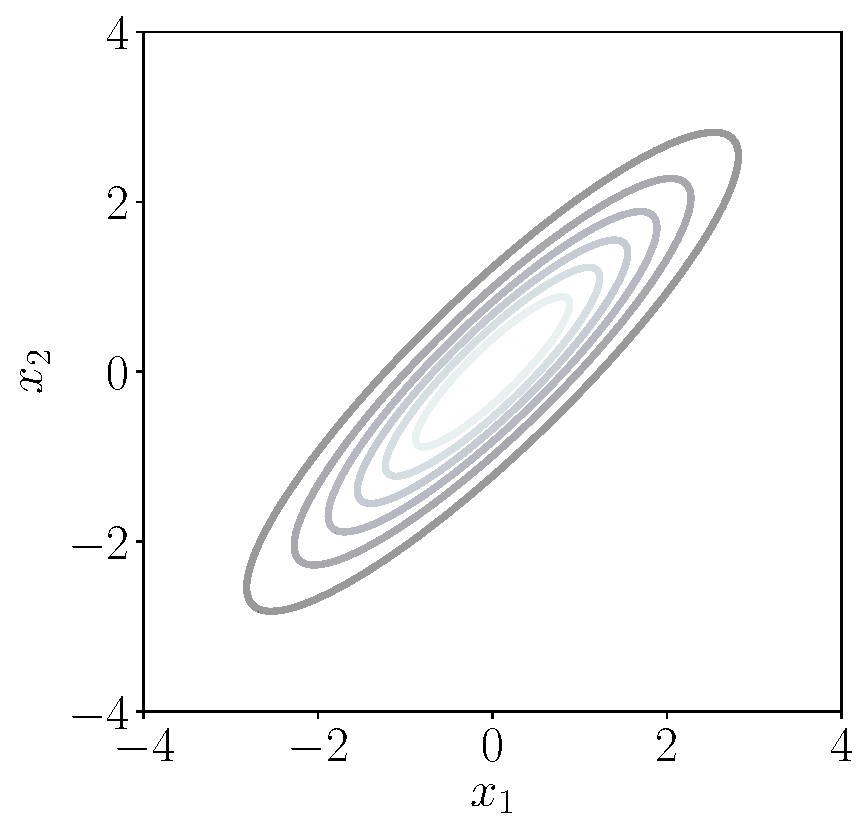
\includegraphics[width=0.4\hsize]{./figures/vi/mean_field_vi_original}%
%     \hspace{5mm}
%     \onslide+<2->{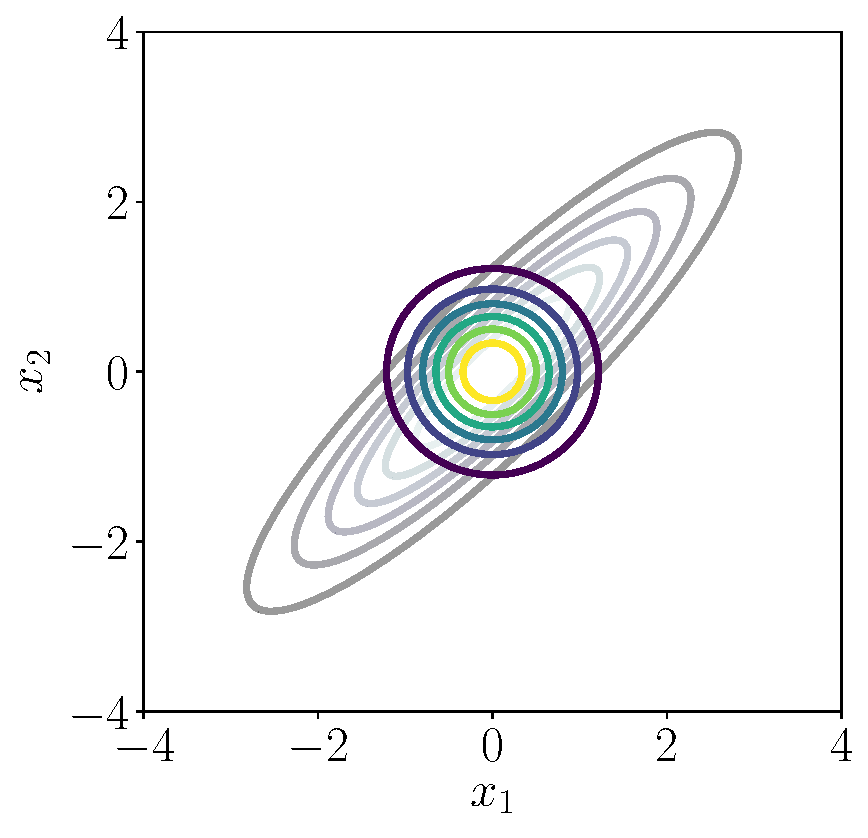
\includegraphics[width=0.4\hsize]{./figures/vi/mean_field_vi_approx}}%
%   \end{center}

%   \begin{itemize}[<+->]
%     \item Mean-field VI to approximate a correlated Gaussian with a
%       factorized Gaussian
%     \item Generally, mean-field VI tends to yield an approximation
%       that is \calert{too compact} \arrow Need better classes of
%       posterior approximations
%   \end{itemize}
% \end{frame}
% %%%%%%%%%%%%%%%%%%%%%%%%%%%%%%%%%%%%%%%%%%%%%
% \begin{frame}{Classical Variational Inference: Limitation}
%   \begin{figure}
%     \centering
%     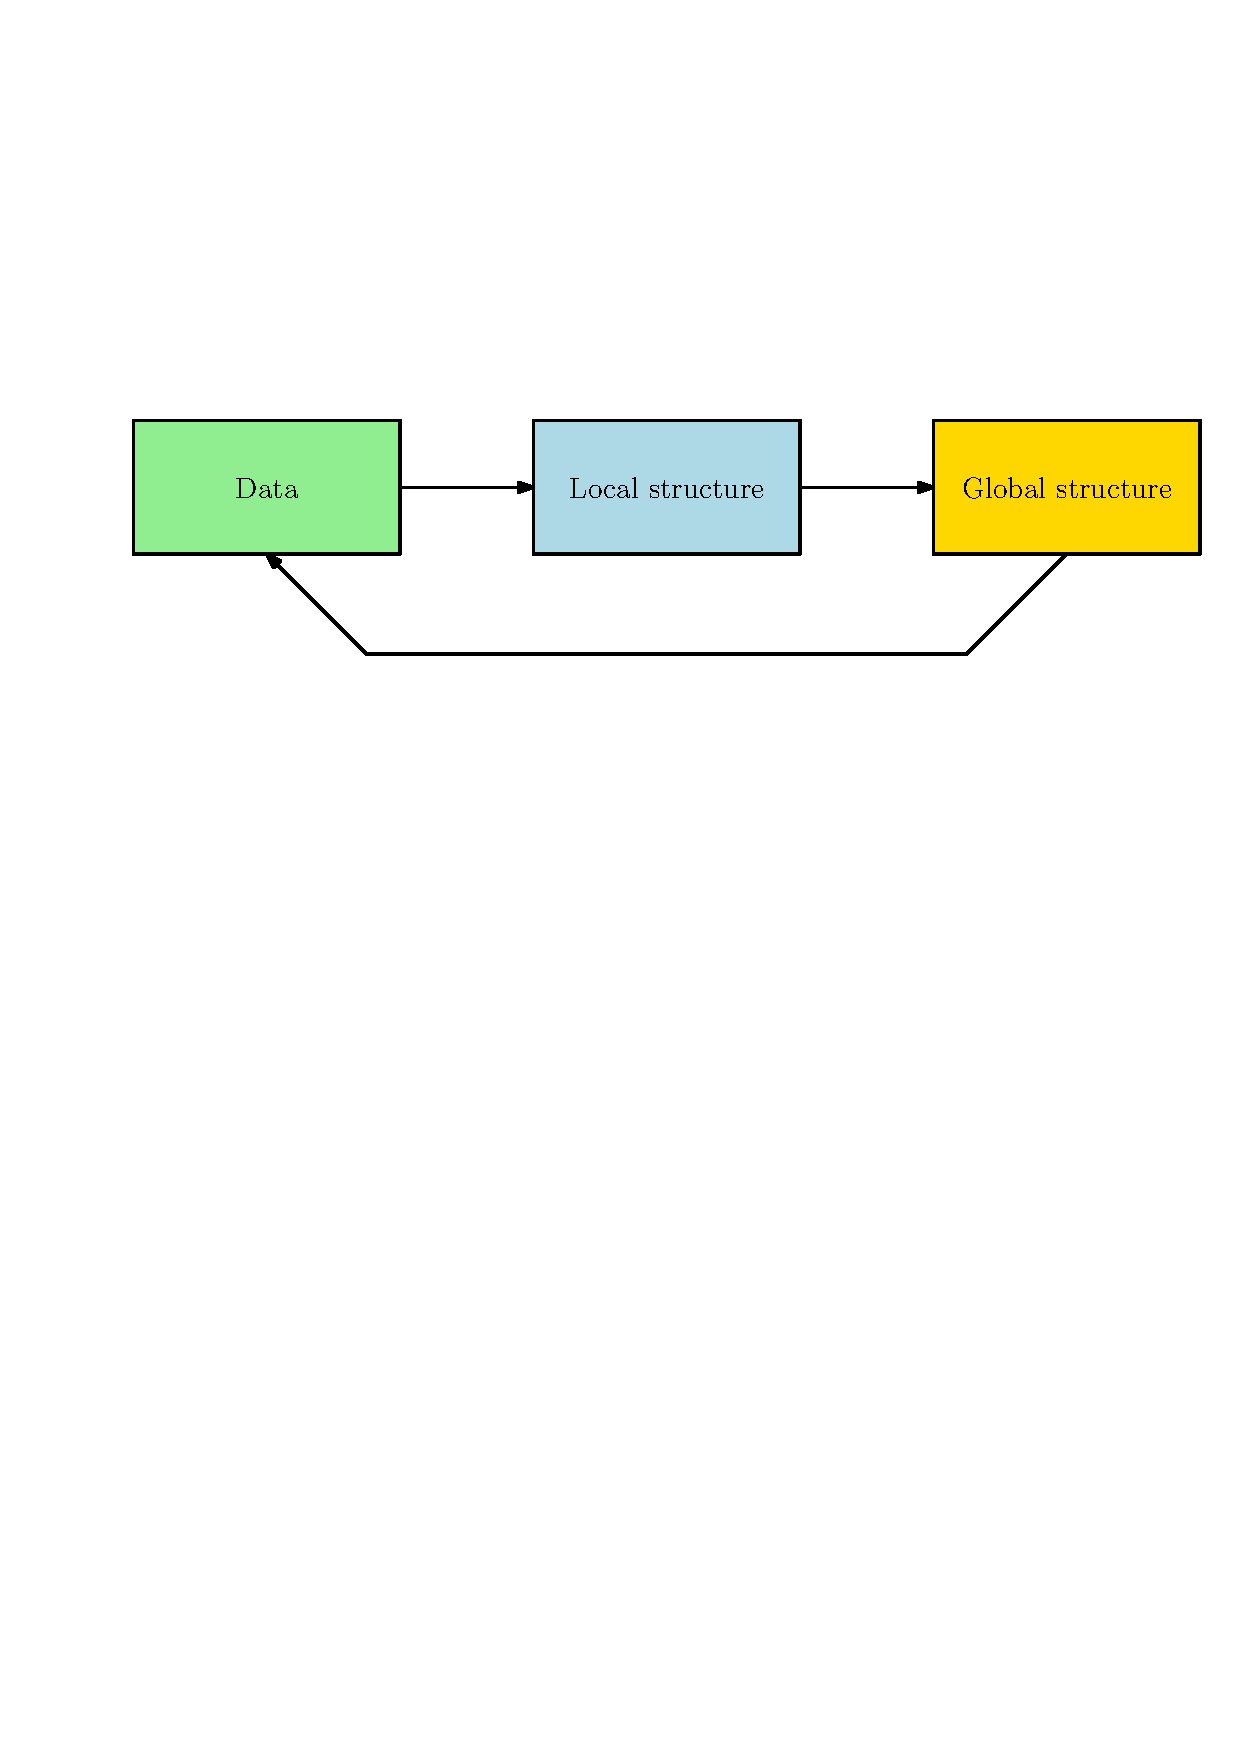
\includegraphics[width=\hsize]{./figures/vi/data_local_global}
%   \end{figure}
%   \pause
%   \begin{itemize}
%   \item Classical VI is inefficient: Need to crunch through the full
%     dataset to update variational parameters\\
%     \alert{Can't handle massive data}
%     \pause
%   \item \emph{Stochastic variational inference} updates the
%     global hidden structure once we have any update of the local
%     structure\\
%     \arrow \cemph{Stochastic optimization}
%   \end{itemize}
% \end{frame}










% \begin{frame}{Some Useful Quantities}
%   \begin{itemize}[<+->]
%   \item \cemph{Kullback-Leibler divergence}
%     \begin{align*}
%     \KL{q(\vec x)}{p(\vec x)} &= \int q(\vec x) \log \frac{q(\vec x)}{p(\vec
%       x)}d\vec x\\
%     &=\E_q\left[\log \frac{q(\vec x)}{p(\vec
%       x)}\right] =  \E_q[\log q(\vec x)] -\E_q[\log p(\vec x)]
%   \end{align*}
% \item \cemph{Differential entropy}
%   $$
%   \mathrm{H}[q(\vec x)] = -\E_q[\log q(\vec x)] = -\int q(\vec x) \log q(\vec
%   x)d\vec x
%   $$
%   \end{itemize}
  
% \end{frame}




% \input{elbo_min_kl}

% \begin{frame}
%   \begin{center}
%     \emph{Evidence Lower Bound}
%   \end{center}
% \end{frame}

% %%%%%%%%%%%%%%%%%%%%%%%%%%%%%%%%%%%%%%%%%%%%%%%%%%%%%%%%
% \input{importance_sampling_recap}
% \input{jensen}
% \input{is2vi}
% \input{elbo}

% %%%%
% \begin{frame}{Overview\phantom{p}}
%    \begin{figure}
%     \centering
%     \scalebox{0.5}{\tikzstyle{ipe stylesheet} = [
  ipe import,
  even odd rule,
  line join=round,
  line cap=butt,
  ipe pen normal/.style={line width=0.4},
  ipe pen heavier/.style={line width=0.8},
  ipe pen fat/.style={line width=1.2},
  ipe pen ultrafat/.style={line width=2},
  ipe pen normal,
  ipe mark normal/.style={ipe mark scale=3},
  ipe mark large/.style={ipe mark scale=5},
  ipe mark small/.style={ipe mark scale=2},
  ipe mark tiny/.style={ipe mark scale=1.1},
  ipe mark normal,
  /pgf/arrow keys/.cd,
  ipe arrow normal/.style={scale=7},
  ipe arrow large/.style={scale=10},
  ipe arrow small/.style={scale=5},
  ipe arrow tiny/.style={scale=3},
  ipe arrow normal,
  /tikz/.cd,
  ipe arrows, % update arrows
  <->/.tip = ipe normal,
  ipe dash normal/.style={dash pattern=},
  ipe dash dashed/.style={dash pattern=on 4bp off 4bp},
  ipe dash dotted/.style={dash pattern=on 1bp off 3bp},
  ipe dash dash dotted/.style={dash pattern=on 4bp off 2bp on 1bp off 2bp},
  ipe dash dash dot dotted/.style={dash pattern=on 4bp off 2bp on 1bp off 2bp on 1bp off 2bp},
  ipe dash normal,
  ipe node/.append style={font=\normalsize},
  ipe stretch normal/.style={ipe node stretch=1},
  ipe stretch normal,
  ipe opacity 10/.style={opacity=0.1},
  ipe opacity 30/.style={opacity=0.3},
  ipe opacity 50/.style={opacity=0.5},
  ipe opacity 75/.style={opacity=0.75},
  ipe opacity opaque/.style={opacity=1},
  ipe opacity opaque,
]
\definecolor{red}{rgb}{1,0,0}%
\definecolor{black}{rgb}{0,0,0}%
\begin{tikzpicture}[ipe stylesheet]
  \draw[shift={(9.892, 640.922)}, xscale=1.3418, yscale=0.5689, ipe
  pen fat]
    (0, 0)
     .. controls (10.6667, 26.6667) and (58.6667, 74.6667) .. (109.3333, 69.3333)
     .. controls (160, 64) and (213.3333, 5.3333) .. (234.6667, -50.6667)
     .. controls (256, -106.6667) and (245.3333, -160) .. (208, -200)
     .. controls (170.6667, -240) and (106.6667, -266.6667) .. (88, -248)
     .. controls (69.3333, -229.3333) and (96, -165.3333) .. (96, -122.6667)
     .. controls (96, -80) and (69.3333, -58.6667) .. (42.6667, -45.3333)
     .. controls (16, -32) and (-10.6667, -26.6667) .. cycle;
  \pic[ipe mark large]
     at (384, 640) {ipe disk};
  \pic[ipe mark large]
     at (176, 608) {ipe disk};
  \draw[ipe pen fat, -{>[ipe arrow large]}]
    (176, 608)
     .. controls (224, 624) and (288, 560) .. (334.0046, 598.8315);
  \draw[red, ipe pen fat]
    (384, 640)
     -- (333.9657, 598.7986);
  \node[ipe node]
     at (150, 650) {\huge{$q(\vec z|\vec \nu)$}};
  \node[ipe node]
     at (160, 580) {\huge{$\vec \nu^{\text{init}}$}};
  \node[ipe node]
     at (310, 590) {\huge{$\vec\nu^{*}$}};
  \node[ipe node]
     at (350, 650) {\huge{$p(\vec z|\vec x)$}};
  \pic[ipe mark large]
  at (334.0046, 598.8315) {ipe disk};
    \node[ipe node, font=\footnotesize]
     at (199.431, 480) {\it \sffamily Figure adopted from Blei et al.'s NIPS-2016 tutorial};
\end{tikzpicture}

%%% Local Variables:
%%% mode: latex
%%% TeX-master: "../lecture_variational_inference"
%%% End:
}
%   \end{figure}
  
%   \begin{itemize}
%   \item Find approximation of a probability distribution (e.g.,
%     posterior) by {optimization}:
%     \begin{enumerate}
%       \item Define an objective function %(will be $\KL{q}{p}$)
%       \item \emph{Define a (parametrized) family of approximating
%         distributions $q_{\vec\nu}$}
%       \item Optimize objective function w.r.t. {variational
%           parameters} $\vec\nu$
%       \end{enumerate}
%      \item Inference \arrow Optimization
%     \end{itemize}
% \end{frame}

% %%%%%%%%%%%%%%%%%%%%%%%%%%%%%%%%%%%%%%%%%%%%%%%
% \begin{frame}{Roadmap I}

%   \begin{enumerate}
%   \item Define a generic class of \cemph{conditionally conjugate models}
%   \item Classical \cemph{mean-field variational inference}
%   \item \cemph{Stochastic variational inference} \arrow Scales to massive data
%   \end{enumerate}
  
% \end{frame}

% \section{Conditionally Conjugate Models}
% \input{generic_model_class}

% %%%%%%%%%%%%%%%%%%%%%%%%%%%%%%%%%%%%%%%%%%%%%%%
% \begin{frame}{Approximating Distributions}

%   \begin{center}
%     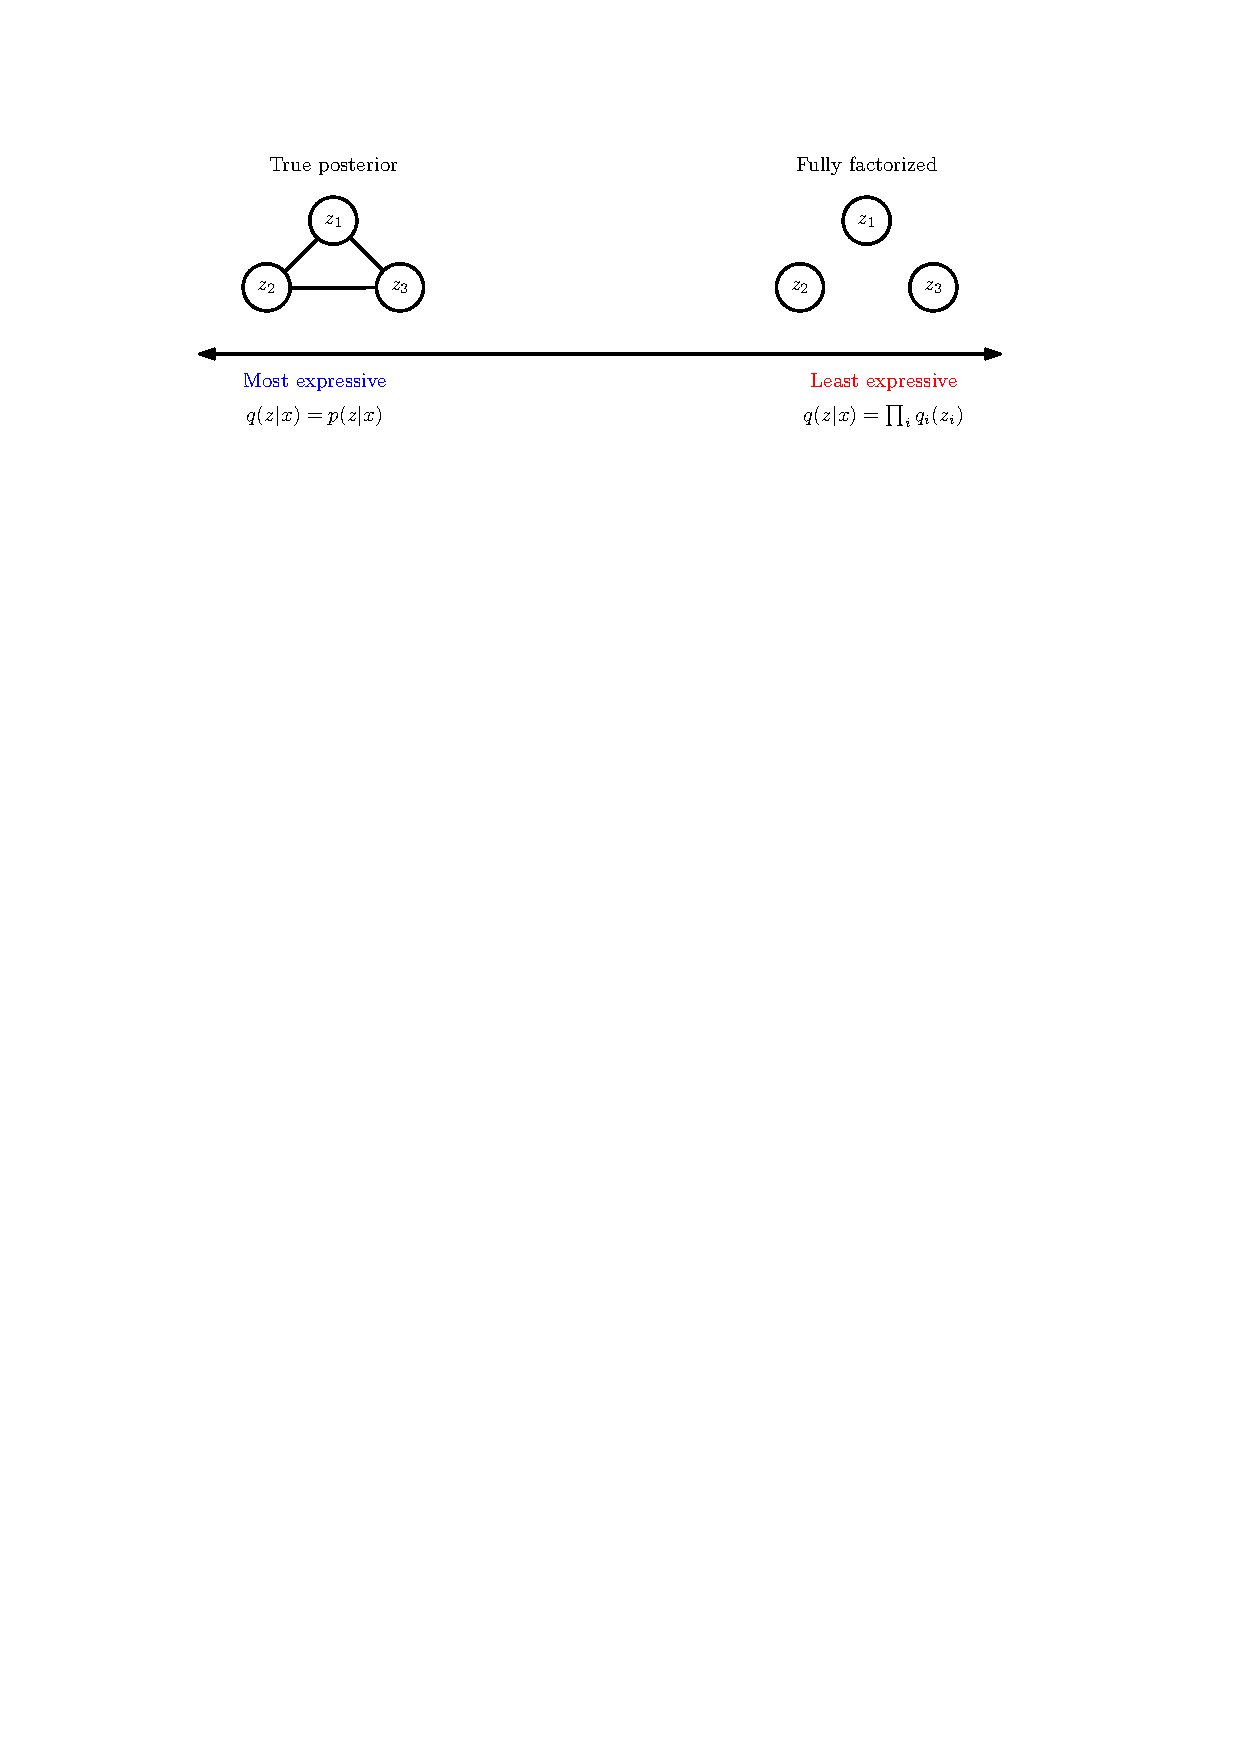
\includegraphics[width=0.85\hsize]{./figures/vi/families_of_q}
%   \end{center}

%   \pause
%   \begin{itemize}
%   \item Specifying the class of posteriors is closely related to
%     specifying a model of the data\\
%     \arrow We have a lot of flexibility \pause
%     \item Generally:
%       \begin{itemize}
%       \item Build \cemph{expressive class of posteriors} (no
%         overfitting problems)
%       \item Maintain \cemph{computational efficiency} \arrow \cemph{Scalability}
%       \end{itemize}
%     \end{itemize}
  
% \end{frame}
% %%%%%%%%%%%%%%%%%%%%%%%%%%%%%%%%%%%%%%%%%%%%%%%
% \section{Mean-Field Variational Inference}
% \input{mean_field_vi}

% \section{Stochastic Variational Inference}
% \input{svi.tex}

% %%%%%%%%%%%%%%%%%%%%%%%%%%%%%%

% \begin{frame}{Overview\phantom{p}}
%    \begin{figure}
%     \centering
%     \scalebox{0.5}{\tikzstyle{ipe stylesheet} = [
  ipe import,
  even odd rule,
  line join=round,
  line cap=butt,
  ipe pen normal/.style={line width=0.4},
  ipe pen heavier/.style={line width=0.8},
  ipe pen fat/.style={line width=1.2},
  ipe pen ultrafat/.style={line width=2},
  ipe pen normal,
  ipe mark normal/.style={ipe mark scale=3},
  ipe mark large/.style={ipe mark scale=5},
  ipe mark small/.style={ipe mark scale=2},
  ipe mark tiny/.style={ipe mark scale=1.1},
  ipe mark normal,
  /pgf/arrow keys/.cd,
  ipe arrow normal/.style={scale=7},
  ipe arrow large/.style={scale=10},
  ipe arrow small/.style={scale=5},
  ipe arrow tiny/.style={scale=3},
  ipe arrow normal,
  /tikz/.cd,
  ipe arrows, % update arrows
  <->/.tip = ipe normal,
  ipe dash normal/.style={dash pattern=},
  ipe dash dashed/.style={dash pattern=on 4bp off 4bp},
  ipe dash dotted/.style={dash pattern=on 1bp off 3bp},
  ipe dash dash dotted/.style={dash pattern=on 4bp off 2bp on 1bp off 2bp},
  ipe dash dash dot dotted/.style={dash pattern=on 4bp off 2bp on 1bp off 2bp on 1bp off 2bp},
  ipe dash normal,
  ipe node/.append style={font=\normalsize},
  ipe stretch normal/.style={ipe node stretch=1},
  ipe stretch normal,
  ipe opacity 10/.style={opacity=0.1},
  ipe opacity 30/.style={opacity=0.3},
  ipe opacity 50/.style={opacity=0.5},
  ipe opacity 75/.style={opacity=0.75},
  ipe opacity opaque/.style={opacity=1},
  ipe opacity opaque,
]
\definecolor{red}{rgb}{1,0,0}%
\definecolor{black}{rgb}{0,0,0}%
\begin{tikzpicture}[ipe stylesheet]
  \draw[shift={(9.892, 640.922)}, xscale=1.3418, yscale=0.5689, ipe
  pen fat]
    (0, 0)
     .. controls (10.6667, 26.6667) and (58.6667, 74.6667) .. (109.3333, 69.3333)
     .. controls (160, 64) and (213.3333, 5.3333) .. (234.6667, -50.6667)
     .. controls (256, -106.6667) and (245.3333, -160) .. (208, -200)
     .. controls (170.6667, -240) and (106.6667, -266.6667) .. (88, -248)
     .. controls (69.3333, -229.3333) and (96, -165.3333) .. (96, -122.6667)
     .. controls (96, -80) and (69.3333, -58.6667) .. (42.6667, -45.3333)
     .. controls (16, -32) and (-10.6667, -26.6667) .. cycle;
  \pic[ipe mark large]
     at (384, 640) {ipe disk};
  \pic[ipe mark large]
     at (176, 608) {ipe disk};
  \draw[ipe pen fat, -{>[ipe arrow large]}]
    (176, 608)
     .. controls (224, 624) and (288, 560) .. (334.0046, 598.8315);
  \draw[red, ipe pen fat]
    (384, 640)
     -- (333.9657, 598.7986);
  \node[ipe node]
     at (150, 650) {\huge{$q(\vec z|\vec \nu)$}};
  \node[ipe node]
     at (160, 580) {\huge{$\vec \nu^{\text{init}}$}};
  \node[ipe node]
     at (310, 590) {\huge{$\vec\nu^{*}$}};
  \node[ipe node]
     at (350, 650) {\huge{$p(\vec z|\vec x)$}};
  \pic[ipe mark large]
  at (334.0046, 598.8315) {ipe disk};
    \node[ipe node, font=\footnotesize]
     at (199.431, 480) {\it \sffamily Figure adopted from Blei et al.'s NIPS-2016 tutorial};
\end{tikzpicture}

%%% Local Variables:
%%% mode: latex
%%% TeX-master: "../lecture_variational_inference"
%%% End:
}
%   \end{figure}
  
%   \begin{itemize}
%   \item Find approximation of a probability distribution (e.g.,
%     posterior) by {optimization}:
%     \begin{enumerate}
%     \item Define an objective function %(will be $\KL{q}{p}$)
%     \item Define a (parametrized) family of approximating
%       distributions $q_{\vec\nu}$
%     \item Optimize objective function w.r.t. {variational parameters}
%       $\vec\nu$
%     \end{enumerate}
%   \item Inference \arrow Optimization
%   \end{itemize}
% \end{frame}



% \begin{frame}{Roadmap II}
%   \begin{enumerate}
%   \item Limits of Classical Variational Inference
%   \item Black-Box Variational Inference
%   \item Computing Gradients of Expectations
%   \end{enumerate}
% \end{frame}

% \section{Limits of Classical Variational Inference}
% \input{limits_vi}
% \section{Black-Box Variational Inference}
%  %%%%%%%%%%%%%%%%%%%%%%%%%%%%%%%%%%%
% \input{bbvi.tex}


% %\section{Computing Gradients of Expectations}
% \section{Computing Gradients of Expectations}

% %%%%%%%%%%%%%%%%%%%%%%%%%%%%%%%%%%%%
% \begin{frame}[t]{Approach}
% \begin{center}
%     \tikzstyle{ipe stylesheet} = [
  ipe import,
  even odd rule,
  line join=round,
  line cap=butt,
  ipe pen normal/.style={line width=0.4},
  ipe pen heavier/.style={line width=0.8},
  ipe pen fat/.style={line width=1.2},
  ipe pen ultrafat/.style={line width=2},
  ipe pen normal,
  ipe mark normal/.style={ipe mark scale=3},
  ipe mark large/.style={ipe mark scale=5},
  ipe mark small/.style={ipe mark scale=2},
  ipe mark tiny/.style={ipe mark scale=1.1},
  ipe mark normal,
  /pgf/arrow keys/.cd,
  ipe arrow normal/.style={scale=7},
  ipe arrow large/.style={scale=10},
  ipe arrow small/.style={scale=5},
  ipe arrow tiny/.style={scale=3},
  ipe arrow normal,
  /tikz/.cd,
  ipe arrows, % update arrows
  <->/.tip = ipe normal,
  ipe dash normal/.style={dash pattern=},
  ipe dash dashed/.style={dash pattern=on 4bp off 4bp},
  ipe dash dotted/.style={dash pattern=on 1bp off 3bp},
  ipe dash dash dotted/.style={dash pattern=on 4bp off 2bp on 1bp off 2bp},
  ipe dash dash dot dotted/.style={dash pattern=on 4bp off 2bp on 1bp off 2bp on 1bp off 2bp},
  ipe dash normal,
  ipe node/.append style={font=\normalsize},
  ipe stretch normal/.style={ipe node stretch=1},
  ipe stretch normal,
  ipe opacity 10/.style={opacity=0.1},
  ipe opacity 30/.style={opacity=0.3},
  ipe opacity 50/.style={opacity=0.5},
  ipe opacity 75/.style={opacity=0.75},
  ipe opacity opaque/.style={opacity=1},
  ipe opacity opaque,
]
\definecolor{red}{rgb}{1,0,0}%
\begin{tikzpicture}[ipe stylesheet]
  \draw[shift={(311.397, 686.186)}, xscale=0.2262, yscale=0.0959]
    (0, 0)
     .. controls (10.6667, 26.6667) and (58.6667, 74.6667) .. (109.3333, 69.3333)
     .. controls (160, 64) and (213.3333, 5.3333) .. (234.6667, -50.6667)
     .. controls (256, -106.6667) and (245.3333, -160) .. (208, -200)
     .. controls (170.6667, -240) and (106.6667, -266.6667) .. (88, -248)
     .. controls (69.3333, -229.3333) and (96, -165.3333) .. (96, -122.6667)
     .. controls (96, -80) and (69.3333, -58.6667) .. (42.6667, -45.3333)
     .. controls (16, -32) and (-10.6667, -26.6667) .. cycle;
  \pic
     at (339.3985, 680.6362) {ipe disk};
  \draw[shift={(339.398, 680.636)}, scale=0.1686, -{>[ipe arrow small]}]
    (0, 0)
     .. controls (48, 16) and (112, -48) .. (158.005, -9.169);
  \pic
     at (366.0336, 679.0905) {ipe disk};
  \node[ipe node]
     at (84, 708) {$p(\vec x, \vec z)$};
  \node[ipe node]
     at (84, 648) {$q(\vec z|\vec \nu)$};
  \draw[shift={(196, 696)}, xscale=1.25,  ipe pen fat]
    (0, 0) rectangle (64, -32);
  \node[ipe node]
     at (204.891, 677.511) {$\displaystyle \int (...) q(\vec z|\vec
       \nu) d\vec z$};
  \node[ipe node]
     at (141.371, 677.339) {$\nabla_{\vec \nu}$};
  \draw[ipe pen fat]
    (132, 696) rectangle (164, 664);
  \draw[->]
    (164, 680)
     -- (196, 680);
  \draw[->]
    (276, 680)
     -- (308, 680);
  \draw[->]
    (112, 656)
     -- (132, 664);
  \draw[->]
    (112, 704)
     -- (132, 696);
  \node[ipe node, font=\tiny]
     at (245, 646.47) {\it \sffamily Adopted from Blei et al.'s NIPS-2016 tutorial};
\end{tikzpicture}

%%% Local Variables:
%%% mode: latex
%%% TeX-master: "../lecture_variational_inference"
%%% End:

%   \end{center}
%   \begin{itemize}
%     \item \emph{Switch order of integration (compute expectations) and
%       differentiation}
%     \item Simplify the expectation after having taken the gradient
%     \end{itemize}
% \end{frame}


% \input{./log_derivative_trick}
% \input{./gradients_of_expectations}


% %%%%%%%%%%%%%%%%%%%%%%%%%%%%%%%%%%%%%%
% \begin{frame}[t]{Approach}
% \begin{center}
%     \tikzstyle{ipe stylesheet} = [
  ipe import,
  even odd rule,
  line join=round,
  line cap=butt,
  ipe pen normal/.style={line width=0.4},
  ipe pen heavier/.style={line width=0.8},
  ipe pen fat/.style={line width=1.2},
  ipe pen ultrafat/.style={line width=2},
  ipe pen normal,
  ipe mark normal/.style={ipe mark scale=3},
  ipe mark large/.style={ipe mark scale=5},
  ipe mark small/.style={ipe mark scale=2},
  ipe mark tiny/.style={ipe mark scale=1.1},
  ipe mark normal,
  /pgf/arrow keys/.cd,
  ipe arrow normal/.style={scale=7},
  ipe arrow large/.style={scale=10},
  ipe arrow small/.style={scale=5},
  ipe arrow tiny/.style={scale=3},
  ipe arrow normal,
  /tikz/.cd,
  ipe arrows, % update arrows
  <->/.tip = ipe normal,
  ipe dash normal/.style={dash pattern=},
  ipe dash dashed/.style={dash pattern=on 4bp off 4bp},
  ipe dash dotted/.style={dash pattern=on 1bp off 3bp},
  ipe dash dash dotted/.style={dash pattern=on 4bp off 2bp on 1bp off 2bp},
  ipe dash dash dot dotted/.style={dash pattern=on 4bp off 2bp on 1bp off 2bp on 1bp off 2bp},
  ipe dash normal,
  ipe node/.append style={font=\normalsize},
  ipe stretch normal/.style={ipe node stretch=1},
  ipe stretch normal,
  ipe opacity 10/.style={opacity=0.1},
  ipe opacity 30/.style={opacity=0.3},
  ipe opacity 50/.style={opacity=0.5},
  ipe opacity 75/.style={opacity=0.75},
  ipe opacity opaque/.style={opacity=1},
  ipe opacity opaque,
]
\definecolor{red}{rgb}{1,0,0}%
\begin{tikzpicture}[ipe stylesheet]
  \draw[shift={(311.397, 686.186)}, xscale=0.2262, yscale=0.0959]
    (0, 0)
     .. controls (10.6667, 26.6667) and (58.6667, 74.6667) .. (109.3333, 69.3333)
     .. controls (160, 64) and (213.3333, 5.3333) .. (234.6667, -50.6667)
     .. controls (256, -106.6667) and (245.3333, -160) .. (208, -200)
     .. controls (170.6667, -240) and (106.6667, -266.6667) .. (88, -248)
     .. controls (69.3333, -229.3333) and (96, -165.3333) .. (96, -122.6667)
     .. controls (96, -80) and (69.3333, -58.6667) .. (42.6667, -45.3333)
     .. controls (16, -32) and (-10.6667, -26.6667) .. cycle;
  \pic
     at (339.3985, 680.6362) {ipe disk};
  \draw[shift={(339.398, 680.636)}, scale=0.1686, -{>[ipe arrow small]}]
    (0, 0)
     .. controls (48, 16) and (112, -48) .. (158.005, -9.169);
  \pic
     at (366.0336, 679.0905) {ipe disk};
  \node[ipe node]
     at (84, 708) {$p(\vec x, \vec z)$};
  \node[ipe node]
     at (84, 648) {$q(\vec z|\vec \nu)$};
  \draw[shift={(196, 696)}, xscale=1.25,  ipe pen fat]
    (0, 0) rectangle (64, -32);
  \node[ipe node]
     at (204.891, 677.511) {$\displaystyle \int (...) q(\vec z|\vec
       \nu) d\vec z$};
  \node[ipe node]
     at (141.371, 677.339) {$\nabla_{\vec \nu}$};
  \draw[ipe pen fat]
    (132, 696) rectangle (164, 664);
  \draw[->]
    (164, 680)
     -- (196, 680);
  \draw[->]
    (276, 680)
     -- (308, 680);
  \draw[->]
    (112, 656)
     -- (132, 664);
  \draw[->]
    (112, 704)
     -- (132, 696);
  \node[ipe node, font=\tiny]
     at (245, 646.47) {\it \sffamily Adopted from Blei et al.'s NIPS-2016 tutorial};
\end{tikzpicture}

%%% Local Variables:
%%% mode: latex
%%% TeX-master: "../lecture_variational_inference"
%%% End:

%   \end{center}
%   \begin{itemize}
%     \item Swap order of integration (compute expectations) and
%       differentiation
%     \item \emph{Simplify the expectation after having taken the
%         gradient}
%     \end{itemize}
% \end{frame}


% \subsection{Score Function Gradients}


% \input{score_function_gradients}
% % \input{control_variates}

% %%%%%%%%%%%%%%%%%%%%%%%%%%%%%%%%%%%%%%%
% \begin{frame}{Non-Conjugate Models}
%   \begin{itemize}
%     \item Nonlinear time series models
%     \item Deep latent Gaussian models
%     \item Attention models (e.g., DRAW)
%     \item Generalized linear models (e.g., logistic regression)
%     \item Bayesian neural networks
%     \item ...
%     \end{itemize}
    

%     \begin{myblock}{}
%       BBVI allows us to design models $p(\vec x, \vec z)$ based
%       on the data, and not on the inference we can do
%     \end{myblock}
%   \end{frame}

% % Now, simplify inference (easier or faster) with some small additional assumptions

%   \subsection{Pathwise Gradients}
% \input{pathwise_gradients}


% % this works nicely for variational inference

% % if you want to put this into the SVI framework we have a computational
% % problem. Amortized inference!

% %%%%%%%%%
% \begin{frame}{Re-cap: Hierarchical Bayesian Models}
%  \begin{center}
%   \begin{tikzpicture}
    \node[latent](z) at (-2,0) {$\vec z_n$};
    \node[obs](x) at (0,0) {$\vec x_n$};
    \node[latent](beta) at (-1,1){$\vec\beta$};
    %\edge{z,mu,sigma}{x};
    \edge{z}{x}
    \edge{beta}{x,z}
    \plate {xz} {(x)(z)} {$n=1,\dotsc, N$} ;
    \node[const] at (-4,0) {\small Local variables};
    \node[const] at (-3.9,1) {\small Global variables};
\end{tikzpicture}
%%% Local Variables:
%%% mode: latex
%%% TeX-master: "../lecture_variational_inference"
%%% End:

% \end{center}

% \begin{itemize}[<+->]
% \item Joint distribution:
% \begin{align*}
% p(\vec\beta,\vec z, \vec x) = p(\vec\beta) \prod_{n=1}^N p(\vec z_n,
%   \vec x_n|\vec\beta)
% \end{align*}
% \item Mean-field variational approximation:
% \begin{center}
%   \scalebox{0.9}{\begin{tikzpicture}
    \node[const](phi) at (-2,0) {\fixgmfont{$\vec\phi_n$}};
    \node[latent](z) at (0,0) {$\vec z_n$};
    \node[latent](beta) at (0,1){$\vec\beta$};
    \node[const](lambda) at (-2,1) {\fixgmfont{$\vec\lambda$}};
    %\edge{z,mu,sigma}{x};
    \edge{lambda}{beta}
    \edge{phi}{z}
    \plate {zphi} {(z)(phi)} {$n=1,\dotsc, N$} ;
\end{tikzpicture}
%%% Local Variables:
%%% mode: latex
%%% TeX-master: "../lecture_variational_inference"
%%% End:
}
% \end{center}
% \end{itemize}


% \end{frame}


% %%%%%%%%%%%%%%%%%%%%%%%%%%%%%%%%%%%%%%%
% \begin{frame}[t]{Re-cap: Mean-Field Stochastic Variational Inference}
%   \begin{enumerate}
%   \item Input: data $\vec x$, model $p(\vec\beta,\vec z, \vec x)$
%   \item Initialize global variational parameters $\vec\lambda$
%     randomly
%   \item Repeat
%   \begin{enumerate}
%     \item Sample data point $\vec x_n$ uniformly at random
%     \item Update local parameter $\vec\phi_n = \E_{\vec\lambda}[...]$
%     \item Compute intermediate global parameter
%       $\hat{\vec\lambda} =  N\E_{\vec\phi_{1:N}}[...]+...$
%     \item Set global parameter
%         $
%         \vec\lambda \leftarrow (1-\rho_t)\vec\lambda +
%         \rho_t\hat{\vec\lambda}
%         $
%     \end{enumerate}
%   \end{enumerate}

% \end{frame}
% %%%%%%%%%%%%%%%%%%%%%%%%%%%%%%%%%%%%%%%
% \begin{frame}[t]{BBVI Stochastic Variational Inference\phantom{p}}
%   \begin{enumerate}
%   \item Input: data $\vec x$, model $p(\vec\beta,\vec z, \vec x)$
%   \item Initialize global variational parameters $\vec\lambda$
%     randomly
%   \item Repeat
%     \begin{enumerate}
%     \item Sample data point $\vec x_n$ uniformly at random
%     \item Update local parameter
%       $\calert{\vec\phi_n = \E_{\vec\lambda}[...]}$
%     \item Compute intermediate global parameter
%       $\calert{\hat{\vec\lambda} = 
%         N\E_{\vec\phi_{1:N}}[...]} + ...$
%     \item Set global parameter
%         $
%         \vec\lambda \leftarrow (1-\rho_t)\vec\lambda +
%         \rho_t\hat{\vec\lambda}
%         $
%     \end{enumerate}
%   \end{enumerate}
% \vspace{-3mm}
%   Issue:
%   \begin{itemize}
%   \item \calert{Expectations} we require to update the local and global
%     parameters are \calert{no longer tractable} \\
%     \arrow No closed-form updating of variational factors
%   \end{itemize}
% \end{frame}

% %%%%%%%%%%%%%%%%%%%%%%%%%%%%%%%%%%%%%%%%%%%%%%%%
% \begin{frame}{Addressing the Challenge}
  
% \begin{itemize}[<+->]
% \item Same problem we had with the ELBO: Integral intractable\\
%   \arrow Gradient descent for variational updates
% \item Idea: Stochastic optimization
% \item Expectations for updating local variational parameters are computed \calert{per data point} \\
%   \arrow
%   Need to run an optimization algorithm per data point\\
%   \arrow \alert{SVI gets really slow}
% \end{itemize}
% \onslide+<4->{\arrow \emph{Amortized Inference}}
% \end{frame}



% \section{Amortized Inference}
% \input{amortized_inference}
% % parametrized function that generates local parameters; parameters of
% % that function are shared

% % we do shrink the class of variational approximations. the more
% % flexible this function the bigger the class

% \input{vae.tex}


% \begin{frame}{Overview}
% \renewcommand{\arraystretch}{1.5}
% \begin{table}[]
% \begin{tabular}{l p{2.5cm} | p{3cm} p{3cm}}
%   & &\multicolumn{2}{c}{Variational approximation of posterior}   \\
%   & & mean-field & more general\\
%   \hline
% \multirow{2}{*}{Model}& conditionally conjugate &
%                                                       \cellcolor[HTML]{9AFF99}
%                                                       analytic solution           &            \\
%                   & hierarchical Bayesian         & \cellcolor[HTML]{FCFF2F}stochastic gradient
%                                             estimators; Example: VAE &
%                                                                        dense
%                                                                        Gaussian,
%                                                                        mixture models,
%                                                                        normalizing
%                                                                        flows,
%                                                                        auxiliary-variable
%                                                                        models\newline
% \end{tabular}
% \end{table}
% \end{frame}


% \section{Richer Posterior Approximations}

% \input{richer_posteriors}




% % % \section{Normalizing Flows}





% %%%%%%%%%%%%%%%%%%%%%%%%%%%%%%%%%%%%%%%%%%%%%%%%%%%%%%%%%%


% \begin{frame}{Summary}
%   \begin{itemize}
%     \item Variational inference \cemph{finds an approximate posterior by
%       optimization}
%       \item \cemph{Minimizing the KL divergence} is equivalent to \cemph{maximizing a
%         lower bound} on the marginal likelihood
%         \item \cemph{Mean-field VI:} analytic updates in conditionally
%           conjugate models
%         \item \cemph{Stochastic VI:} Stochastic optimization for scalability
%         \item General models require us to compute \cemph{gradients of
%           expectations}
%           \begin{itemize}
%           \item Score-function gradients
%             \item Pathwise gradients
%             \end{itemize}
%           \item \cemph{Amortized inference}
%             \item Modern VI allows us to specify \cemph{rich classes of
%               posterior approximations}
%   \end{itemize}
% \end{frame}


%%%%%%%%%%%%%%%%%%%%%%%%%%%%%%%%%%%%%%%%%
% REFERENCES
%%%%%%%%%%%%%%%%%%%%%%%%%%%%%%%%%%%%%%%%%
\begin{frame}[t,allowframebreaks]
\frametitle{References}
\linespread{1.0}
\tiny
\bibliographystyle{abbrv}
\bibliography{../includes/pi-literature}
\end{frame}



\end{document}
%%% Local Variables: 
%%% mode: latex
%%% TeX-master: t
%%% End: 
